\documentclass[11pt,oneside]{article}
\usepackage[a4paper,margin=25mm,headheight=15pt]{geometry}
\usepackage[T1]{fontenc}
\usepackage[utf8]{inputenc}
\IfFileExists{libertinus.sty}{\usepackage{libertinus}}{\usepackage{lmodern}}
\usepackage{microtype}
\usepackage{amsmath,amssymb,amsthm,mathtools,mathrsfs,bm}
\usepackage{booktabs,longtable,array,tabularx,multirow}
\usepackage{graphicx}
\usepackage{caption}
\usepackage{xcolor}
\usepackage{enumitem}
\usepackage{fancyhdr}
\usepackage{titlesec}
\usepackage{listings}
\usepackage{xurl}
\usepackage[hypertexnames=false]{hyperref}
\usepackage[nameinlink,noabbrev]{cleveref}
\usepackage{aliascnt}

\graphicspath{{figures/}}
\definecolor{linkblue}{RGB}{31,78,121}
\definecolor{deepgreen}{RGB}{35,105,78}
\definecolor{shadegray}{RGB}{246,247,249}
\definecolor{rulegray}{RGB}{194,201,208}
\hypersetup{
  colorlinks=true,
  linkcolor=linkblue,
  citecolor=deepgreen,
  urlcolor=linkblue,
  pdftitle={Closing the Rvachev--Lagrange Loop},
  pdfsubject={Exact fixed-radius up-function synthesis of Lagrange polynomials and coefficient-space projectors},
  pdfkeywords={Rvachev up-function, Fabius function, Lagrange interpolation, Strang--Fix, Appell polynomials, Bernoulli numbers, Bell polynomials, Thue--Morse, oblique projector, Runge phenomenon}
}

\pagestyle{fancy}
\fancyhf{}
\fancyhead[L]{\small Closing the Rvachev--Lagrange loop}
\fancyhead[R]{\small\nouppercase{\leftmark}}
\fancyfoot[C]{\thepage}
\renewcommand{\headrulewidth}{0.4pt}
\titleformat{\section}{\Large\bfseries}{\thesection}{0.7em}{}
\titleformat{\subsection}{\large\bfseries}{\thesubsection}{0.7em}{}
\titleformat{\subsubsection}{\normalsize\bfseries}{\thesubsubsection}{0.7em}{}
\setcounter{secnumdepth}{3}
\setcounter{tocdepth}{2}
\setlist[itemize]{leftmargin=2em,itemsep=0.25em,topsep=0.4em}
\setlist[enumerate]{leftmargin=2.3em,itemsep=0.25em,topsep=0.4em}
\setlength{\emergencystretch}{3em}
\allowdisplaybreaks[2]
\numberwithin{equation}{section}

\newtheorem{theorem}{Theorem}[section]
\newcommand{\newsharedtheorem}[2]{%
  \newaliascnt{#1}{theorem}%
  \newtheorem{#1}[#1]{#2}%
  \aliascntresetthe{#1}%
}
\newsharedtheorem{proposition}{Proposition}
\newsharedtheorem{lemma}{Lemma}
\newsharedtheorem{corollary}{Corollary}
\newsharedtheorem{identity}{Identity}
\newsharedtheorem{conjecture}{Conjecture}
\newsharedtheorem{problem}{Problem}
\newsharedtheorem{question}{Research question}
\theoremstyle{definition}
\newsharedtheorem{definition}{Definition}
\newsharedtheorem{algorithm}{Algorithm}
\newsharedtheorem{example}{Example}
\newsharedtheorem{observation}{Numerical observation}
\theoremstyle{remark}
\newsharedtheorem{remark}{Remark}
\newsharedtheorem{warning}{Warning}
\crefname{conjecture}{conjecture}{conjectures}
\Crefname{conjecture}{Conjecture}{Conjectures}
\crefname{problem}{problem}{problems}
\Crefname{problem}{Problem}{Problems}
\crefname{question}{research question}{research questions}
\Crefname{question}{Research question}{Research questions}
\crefname{observation}{numerical observation}{numerical observations}
\Crefname{observation}{Numerical observation}{Numerical observations}
\crefname{identity}{identity}{identities}
\Crefname{identity}{Identity}{Identities}
\crefname{algorithm}{algorithm}{algorithms}
\Crefname{algorithm}{Algorithm}{Algorithms}

\newcommand{\eps}{\varepsilon}
\newcommand{\Ran}{\operatorname{Ran}}
\newcommand{\Ker}{\operatorname{Ker}}
\newcommand{\tr}{\operatorname{tr}}
\newcommand{\PiN}{\mathcal P}
\newcommand{\App}{\mathscr A}
\newcommand{\MGF}{\mathsf M}
\newcommand{\Lag}{\mathcal I}
\newcommand{\Eval}{\mathcal E}
\newcommand{\Rec}{\mathcal L}
\newcommand{\Synth}{\mathcal R}
\newcommand{\Coeff}{\mathcal S}
\newcommand{\Proj}{\mathsf P}
\newcommand{\Bell}{Y}
\newcommand{\repo}{\nolinkurl{Analysis/FabiusFunction/docs}}

\newenvironment{statusbox}[1]{%
  \par\smallskip\noindent\begin{center}\begin{minipage}{0.94\textwidth}%
  \hrule\vspace{0.5em}\noindent\textbf{#1}\par\smallskip
}{%
  \vspace{0.5em}\hrule\end{minipage}\end{center}\smallskip
}

\lstdefinestyle{pythonstyle}{
  language=Python,
  basicstyle=\ttfamily\footnotesize,
  backgroundcolor=\color{shadegray},
  frame=single,
  rulecolor=\color{rulegray},
  columns=fullflexible,
  keepspaces=true,
  showstringspaces=false,
  breaklines=true,
  xleftmargin=0.7em,
  xrightmargin=0.7em,
  aboveskip=0.8em,
  belowskip=0.8em
}

\title{\bfseries Closing the Rvachev--Lagrange Loop\\[0.45em]
\large Exact fixed-radius polynomial synthesis, signed Markov decoders,\\
coefficient-space projectors, and dyadic spectral multiplicities}
\author{Research report for Vladimir Reshetnikov's \texttt{ProveIt} project}
\date{29 August 2026}

\begin{document}
\maketitle

\begin{abstract}
Let $u=\RvachevUp$ be Rvachev's compactly supported $C^\infty$ function,
normalized as an even probability density on $[-1,1]$.  The repository volume
\emph{Exact Polynomial Synthesis by Finite Rvachev Up-Function Dictionaries}
proves that the integer-shift system generated by a scale-$2^n$ copy of $u$
reproduces every polynomial of degree at most $n$, with coefficients obtained
by finite inverse-moment Appell deconvolution.  Affine conjugation turns that
result into the fixed-physical-radius identity
\[
 p(x)=2^{-n}\sum_{k=-2^{n+1}+1}^{2^{n+1}-1}
 \bigl[\MGF_u(D)^{-1}p\bigr](k2^{-n})\,u(x-k2^{-n}),
 \qquad -1\le x\le1,
\]
for every $p\in\PiN_n$.  Thus the atoms are literal translates of the
\emph{same} $u$; no dilation remains.  Applied to the Lagrange cardinal
polynomials $\ell_j$, this gives a completely explicit finite representation,
whose coefficients are rational combinations of Bernoulli numbers, complete
Bell polynomials, and elementary symmetric polynomials of the shifted nodes.

Substituting these formulas into the Lagrange interpolant of $u$ closes the
loop.  The resulting up-shift sum is not a new approximation operator in
disguise: at every fixed degree it factors the ordinary interpolation
projector exactly.  In operator notation,
\[
 \Lag_n=\Synth_n\,C_n\,\Eval_n,
 \qquad B_nC_n=I_{n+1},
 \qquad \Proj_n=C_nB_n,
\]
where $C_n$ converts nodal data to up-amplitudes and $B_n$ samples an
up-dictionary at the interpolation nodes.  After a natural normalization,
$B_n$ is a positive row-stochastic matrix and the Appell--Lagrange decoder is
a signed row-stochastic right inverse.  Consequently $\Proj_n$ is an exact
oblique projector with eigenvalue $1$ of multiplicity $n+1$ and eigenvalue
$0$ of multiplicity $4\cdot2^n-n-2$.  Its zero eigenspace splits into an
explicit Thue--Morse/$2$-adic alias sector of dimension $2^{n+1}-n-2$ and a
sample-invisible local-spline sector of dimension $2^{n+1}$.  Nested node
sets lift to a commuting flag of coefficient projectors; for dyadic degrees
$n_q=2^q$, the detail idempotents have eigenvalue-$1$ multiplicities
$2^{q-1}$.

The factorization proves an exact transfer principle: every finite truncation
error inside a level is zero, and the infinite up-shift series converges,
diverges, or exhibits Runge oscillation precisely when the underlying
Lagrange series does.  Chebyshev--Lobatto levels therefore give
superalgebraic convergence for $u$, while the equispaced loop inherits the
repository's Runge instability.  Exact rational computations verify the
right-inverse identity through degree $8$; reduced-QR experiments show the
projector norm growing from $2.19$ at degree $2$ to $3.02\times10^3$ at
degree $12$ for equispaced nodes, versus $1.11\times10^2$ for Chebyshev
nodes.  A concrete first closed loop is
\[
 1-x^2=\sum_{k=-7}^{7}\left(\frac5{18}-\frac{k^2}{64}\right)
 u\!\left(x-\frac{k}{4}\right),\qquad -1\le x\le1.
\]
The report ends with conjectures on fixed-radius complexity, projector
obliquity, minimal-variation alias gauges, and Lambert-$W$/log-periodic
asymptotics of the equispaced boundary layer.
\end{abstract}

\clearpage
\tableofcontents
\clearpage

\section{Corpus audit, provenance, and novelty boundary}
\label{sec:corpus}

The analysis uses the recursive documentation snapshot of
\texttt{VladimirReshetnikov/ProveIt} at commit
\begin{center}
\nolinkurl{4544e9af6b94820402c69967be1dff3f85e43c1e}
\end{center}
from 29 August 2026.  The current tree contains 65 \TeX{} documents under
\repo, including the living exposition, archived derivations, seven paper
transcriptions, the Lean walkthrough, the twelve-document Fourier-decay
corpus, and the large consolidated frontier volumes.  The audit treated
archived files as mathematical sources while mapping frozen or absorbed
copies to their current canonical expositions.

The two directly controlling documents are:
\begin{enumerate}
\item \emph{Exact Polynomial Synthesis by Finite Rvachev Up-Function
Dictionaries} (the current
\nolinkurl{drafts/representations/Up_Polynomial_Synthesis/} volume), which
proves the scale classification, global Appell deconvolution formula, exact
local dimensions, dyadic alias annihilator, endpoint basis, and
output-sensitive coefficient algorithm;
\item \emph{Dyadic-Comb Frontiers for the Fabius--Rvachev System} (the current
\nolinkurl{drafts/inverse-and-sampling/comb-interpolation/Dyadic_Comb_Frontiers/} volume), which
sets up global Lagrange interpolation of $F$ and $u$, exact symmetry
compressions, endpoint-flat Hermite variants, and the Runge/stability study.
\end{enumerate}
The primary exposition supplies the normalization of $F$ and $u$, the
Fourier sinc product, functional equations, moments, and exact dyadic values.
The representation, exponent/$q$-series, Thue--Morse, inverse/sampling,
spectral/arithmetic, and Fourier-decay frontier volumes were checked for
nearby formulas and for possible duplication.

\begin{statusbox}{What is imported, and what is new here}
The scale-$2^n$ polynomial-synthesis theorem, its Appell coefficient
operator, the annihilator
$A_n(z)=\prod_{r=1}^{n}[2^r]_z$, and the local-dimension theorem are imported
from the synthesis volume.  The ordinary interpolation projector and its
Runge analysis are imported from the dyadic-comb volume.  The contribution
of this report is their affine fixed-radius specialization and systematic
composition: the explicit Lagrange-cardinal transform, the exact loop
factorization, the stochastic/right-inverse normalization, the coefficient
projector and its spectral ledger, the function-space direct sum and exact
sequence, the nested dyadic projector flag, the decoder-sign/variation
bounds, and the associated convergence and stability transfer principles.
Searches of the pinned corpus for ``coefficient-space projector'' and
``self-representation operator'' found no pre-existing treatment.  Novelty
claims below are therefore relative to this audited repository snapshot, not
unqualified claims of world priority.
\end{statusbox}

The classical fact that atomic-function spaces contain polynomials goes back
to the Rvachevs~\cite{RvachevRvachev1972,Rvachev1990}.  The present formulas
also sit naturally within Strang--Fix theory and the theory of principal
shift-invariant spaces~\cite{StrangFix1973,deBoorRon1992,deBoorDeVoreRon1994}.

\section{Notation and imported structural facts}
\label{sec:prelim}

\subsection{The up-function as a probability density}

Throughout, $u=\RvachevUp$ is even, nonnegative, supported on $[-1,1]$, and
normalized by
\begin{equation}
 \int_{-1}^{1}u(x)\Differential x=1,
 \qquad u(0)=1,
 \qquad u(\pm1)=0.
 \label{eq:up-normalization}
\end{equation}
With the Fourier convention
$\widehat f(\xi)=\int_{\RealNumbers}f(x)\EulerE^{-2\pi\ImaginaryUnit x\xi}\Differential x$,
\begin{equation}
 \widehat u(\xi)=\prod_{j\ge0}\SincPi\!\left(\frac{\xi}{2^j}\right),
 \qquad
 \operatorname{ord}_{\xi=q}\widehat u=1+\TwoAdicValuation(q)
 \quad(q\in\IntegerNumbers\setminus\{0\}).
 \label{eq:fourier-product}
\end{equation}
Equivalently, if
$Z=\sum_{j\ge1}2^{-j}V_j$ with independent
$V_j\sim\operatorname{Unif}[-1,1]$, then $u$ is the density of $Z$.
Its moment generating function is
\begin{equation}
 \MGF_u(z)=\mathbb E\EulerE^{zZ}
 =\prod_{j\ge1}\frac{\sinh(z/2^j)}{z/2^j}.
 \label{eq:mgf}
\end{equation}
The logarithm has even cumulants
\begin{equation}
 \log\MGF_u(z)=\sum_{r\ge1}\kappa_{2r}\frac{z^{2r}}{(2r)!},
 \qquad
 \kappa_{2r}=\frac{B_{2r}}{2r(1-4^{-r})},
 \qquad \kappa_{2r+1}=0.
 \label{eq:cumulants}
\end{equation}

\subsection{The inverse-moment Appell operator}

Define rational numbers $\gamma_r$ by
\begin{equation}
 \frac1{\MGF_u(z)}=\sum_{r\ge0}\gamma_r\frac{z^r}{r!}
 =\exp\!\left(-\sum_{s\ge1}\kappa_{2s}
                     \frac{z^{2s}}{(2s)!}\right).
 \label{eq:gamma-egf}
\end{equation}
Thus $\gamma_{2r+1}=0$ and
\begin{equation}
 \gamma_0=1,
 \quad \gamma_2=-\frac19,
 \quad \gamma_4=\frac{31}{675},
 \quad \gamma_6=-\frac{2347}{59535},
 \quad \gamma_8=\frac{1904369}{32531625}.
 \label{eq:gamma-first}
\end{equation}
The complete Bell-polynomial formula is
\begin{equation}
 \gamma_r=\Bell_r(-\kappa_1,-\kappa_2,\ldots,-\kappa_r),
 \label{eq:gamma-bell}
\end{equation}
or, more explicitly,
\begin{equation}
 \frac{\gamma_{2r}}{(2r)!}
 =\sum_{\substack{k_1+2k_2+\cdots+rk_r=r\\k_s\ge0}}
   \prod_{s=1}^{r}\frac1{k_s!}
   \left(-\frac{\kappa_{2s}}{(2s)!}\right)^{k_s}.
 \label{eq:gamma-partition}
\end{equation}
For a polynomial $p$ define the terminating differential operator
\begin{equation}
 \App p:=\MGF_u(D)^{-1}p
 =\sum_{r=0}^{\Floor{\deg p/2}}
   \frac{\gamma_{2r}}{(2r)!}\,p^{(2r)}.
 \label{eq:App-operator}
\end{equation}
The deconvolution Appell polynomials are
\begin{equation}
 \mathcal A_r(y):=\App(y^r)
 =\sum_{s=0}^{r}\binom rs\gamma_s y^{r-s},
 \qquad \mathcal A_r'(y)=r\mathcal A_{r-1}(y).
 \label{eq:Appell-polynomials}
\end{equation}
The operator is triangular with unit diagonal on every polynomial space;
hence it is an automorphism of $\PiN_n$.

\subsection{Lagrange interpolation}

Let $X_n=\{x_0,\ldots,x_n\}\subset[-1,1]$ consist of distinct nodes and put
\begin{equation}
 \omega_n(x)=\prod_{j=0}^{n}(x-x_j),
 \qquad
 \ell_j(x)=\frac{\omega_n(x)}{(x-x_j)\omega_n'(x_j)}.
 \label{eq:lagrange-cardinal}
\end{equation}
Then $\ell_j(x_i)=\delta_{ij}$ and
\begin{equation}
 (\Lag_nf)(x)=\sum_{j=0}^{n}f(x_j)\ell_j(x)
 \label{eq:interpolant}
\end{equation}
projects functions onto $\PiN_n$.  We distinguish the evaluation map
$\Eval_n f=(f(x_0),\ldots,f(x_n))^T$ from the reconstruction map
$\Rec_n y=\sum_jy_j\ell_j$, so
\begin{equation}
 \Lag_n=\Rec_n\Eval_n,
 \qquad \Eval_n\Rec_n=I_{n+1}.
 \label{eq:Lagrange-factor}
\end{equation}

\section{Affine conjugation: exact synthesis by literal shifts}
\label{sec:fixed-radius}

The synthesis volume works with the normalized atoms
\begin{equation}
 \psi_{\rho,k}(t)=\frac1\rho u\!\left(\frac{t-k}{\rho}\right).
 \label{eq:normalized-atoms}
\end{equation}
For integer $\rho$, their Strang--Fix reproduction degree is exactly
$\TwoAdicValuation(\rho)$, because the least multiplicity of a nonzero dual-lattice zero
of $\widehat u(\rho\xi)$ is $1+\TwoAdicValuation(\rho)$.  The smallest common scale that
reproduces $\PiN_n$ is therefore $m=2^n$.

\begin{theorem}[Canonical fixed-radius polynomial synthesis]
\label{thm:fixed-radius}
Let $p\in\PiN_n$, put
\begin{equation}
 m=2^n,
 \qquad h=m^{-1}=2^{-n},
 \qquad K_n=\{-2m+1,-2m+2,\ldots,2m-1\}.
 \label{eq:m-h-K}
\end{equation}
Then the global locally finite identity
\begin{equation}
 \boxed{
 p(x)=h\sum_{k\in\IntegerNumbers}(\App p)(kh)\,u(x-kh)
 }
 \label{eq:global-fixed-radius}
\end{equation}
holds for every $x\in\RealNumbers$.  On $[-1,1]$ it reduces exactly to the finite sum
\begin{equation}
 \boxed{
 p(x)=h\sum_{k\in K_n}(\App p)(kh)\,u(x-kh),
 \qquad -1\le x\le1.
 }
 \label{eq:finite-fixed-radius}
\end{equation}
Thus $4m-1=4\cdot2^n-1$ literal translates of the same unscaled $u$ form a
canonical finite dictionary for every degree-$n$ polynomial on $[-1,1]$.
\end{theorem}

\begin{proof}
The imported global synthesis theorem says that for $P\in\PiN_n$,
\begin{equation}
 P(t)=\frac1m\sum_{k\in\IntegerNumbers}Q(k)
 u\!\left(\frac{t-k}{m}\right),
 \qquad
 Q=\MGF_u(mD_t)^{-1}P.
 \label{eq:imported-global}
\end{equation}
Set $P(t)=p(t/m)$ and then $t=mx$.  Since
$D_t^rP(t)=m^{-r}p^{(r)}(t/m)$,
\[
 Q(t)=\sum_r\gamma_r\frac{m^rD_t^rP(t)}{r!}
     =(\App p)(t/m).
\]
Substitution in \eqref{eq:imported-global} gives
\eqref{eq:global-fixed-radius}.  If $x\in[-1,1]$, the factor
$u(x-kh)$ can be nonzero only when $kh\in[x-1,x+1]\subset[-2,2]$.
The boundary indices $k=\pm2m$ contribute $u(\pm1)=0$, leaving exactly
$K_n$.
\end{proof}

\begin{remark}[Why this is genuinely a no-dilation formula]
The exponential scale $m=2^n$ has not disappeared; it has moved from the
\emph{shape} to the \emph{spacing}.  In the original variable, the atom is
$u((t-k)/m)$.  Under $t=mx$, it becomes $u(x-k/m)$: the support radius is
literally one, while the grid spacing is $h=2^{-n}$.  This is precisely the
physical-radius-$\rho=1$ regime requested in the problem.
\end{remark}

\begin{corollary}[Monomial reproduction]
\label{cor:monomial}
For $0\le r\le n$,
\begin{equation}
 x^r=h\sum_{k\in K_n}\mathcal A_r(kh)u(x-kh),
 \qquad -1\le x\le1.
 \label{eq:monomial-reproduction}
\end{equation}
In particular,
\begin{align}
 1&=h\sum_{k\in K_n}u(x-kh),
 \label{eq:partition-unity}\\
 x&=h\sum_{k\in K_n}(kh)u(x-kh),
 \label{eq:first-moment}\\
 x^2&=h\sum_{k\in K_n}\left((kh)^2-\frac19\right)u(x-kh).
 \label{eq:second-moment}
\end{align}
\end{corollary}

The first identity says that the oversampled translates form a partition of
unity after multiplication by $h$; it will turn the collocation matrix into a
Markov matrix in \cref{sec:operators}.

\subsection{A compressed but asymmetric unscaled basis}

The canonical formula \eqref{eq:finite-fixed-radius} is redundant.  The
multi-cell dimension theorem in the synthesis volume yields a smaller
unscaled basis after the same physical specialization.

\begin{theorem}[Alias-compressed fixed-radius basis]
\label{thm:compressed-basis}
With $m=2^n$ and $h=1/m$, define
\begin{equation}
 \tau_r=-(n+1)h+rh,
 \qquad 0\le r\le2m+n.
 \label{eq:compressed-centers}
\end{equation}
The $2m+n+1$ functions $u(x-\tau_r)$ restrict to a basis of the complete
local shift space generated on $[-1,1]$ by all active $h\IntegerNumbers$-translates.
Every $p\in\PiN_n$ therefore has a unique representation in this basis.  A
reflected left-end basis is obtained by $x\mapsto-x$.
\end{theorem}

\begin{proof}
Apply the imported physical multi-cell theorem with interval $[a,b]=[-1,1]$,
polynomial degree $n$, scale parameter $M=m$, and $J=2m$ cells.  Then
$h=(b-a)/J=1/m$ and the physical atom radius is $Mh=1$.  The theorem's basis
centers are
\[
 a+h(M-n-1+r)=-1+\frac{m-n-1+r}{m}=-(n+1)h+rh.
\]
After which its dimension formula gives $J+n+1=2m+n+1$.
\end{proof}

The coefficient reduction from $4m-1$ to $2m+n+1$ is governed by the dyadic
alias annihilator
\begin{equation}
 A_n(z)=\prod_{r=1}^{n}[2^r]_z
 =\prod_{r=1}^{n}\frac{1-z^{2^r}}{1-z}
 =\prod_{\ell=1}^{n}(z^{2^{\ell-1}}+1)^{n-\ell+1}.
 \label{eq:annihilator}
\end{equation}
Its degree is $2m-n-2$, exactly the number of dense-dictionary aliases
eliminated.  This is where the $q$-integer and Thue--Morse structure enters
the fixed-radius problem.

\begin{proposition}[Optimal uniform-lattice spacing]
\label{prop:lattice-optimal}
Among uniform lattices $h\IntegerNumbers$ for which $1/h$ is an integer, global
reproduction of $\PiN_n$ by unscaled translates $u(x-kh)$ requires
$h\le2^{-n}$.  Hence the grid in \cref{thm:fixed-radius} is the coarsest
uniform integer-ratio grid with degree-$n$ Strang--Fix order.
\end{proposition}

\begin{proof}
Rescale by $t=x/h$.  The generator becomes $u((t-k)/\rho)$ with
$\rho=1/h$.  The imported scale classification gives reproduction degree
$\TwoAdicValuation(\rho)$, so $\TwoAdicValuation(1/h)\ge n$ and therefore $1/h$ is divisible by
$2^n$.
\end{proof}

\section{Lagrange cardinal polynomials as finite up-shift combinations}
\label{sec:lagrange-synthesis}

The fixed-radius theorem may now be applied one cardinal at a time.  This is
the requested representation on $[-1,1]$.

\begin{theorem}[Canonical up-shift representation of the Lagrange basis]
\label{thm:lagrange-up}
For each $0\le j\le n$ and every $x\in[-1,1]$,
\begin{equation}
 \boxed{
 \ell_j(x)=h\sum_{k\in K_n}D_{kj}^{(n)}u(x-kh),
 \qquad
 D_{kj}^{(n)}:=(\App\ell_j)(kh).
 }
 \label{eq:lagrange-up}
\end{equation}
Equivalently,
\begin{equation}
 D_{kj}^{(n)}
 =\sum_{r=0}^{\Floor{n/2}}
   \frac{\gamma_{2r}}{(2r)!}\ell_j^{(2r)}(kh).
 \label{eq:D-derivative}
\end{equation}
All sums are finite.  If the nodes are rational, every coefficient is
rational.
\end{theorem}

\begin{proof}
Apply \cref{thm:fixed-radius} to $p=\ell_j$.  Formula
\eqref{eq:D-derivative} is the terminating definition of $\App$.
Rationality follows from the rational Bernoulli numbers, hence rational
$\gamma_{2r}$, and from the rational coefficients of a Lagrange cardinal at
rational nodes.
\end{proof}

\subsection{A closed coefficient formula in elementary symmetric polynomials}

The derivative form is already constructive, but it admits a compact
node-symmetric expression.  For a finite multiset $Y$, let $e_r(Y)$ denote
the elementary symmetric polynomial of degree $r$, with $e_0=1$ and
$e_r=0$ outside the natural range.

\begin{proposition}[Bernoulli--Appell--symmetric coefficient formula]
\label{prop:symmetric-coeff}
Let $t_k=kh$.  Then
\begin{equation}
 \boxed{
 D_{kj}^{(n)}=
 \frac{1}{\omega_n'(x_j)}
 \sum_{r=0}^{\Floor{n/2}}\gamma_{2r}\,
 e_{n-2r}\bigl(\{t_k-x_s:s\ne j\}\bigr).
 }
 \label{eq:D-elementary}
\end{equation}
Consequently every coefficient is a finite Bell--Bernoulli polynomial in the
cumulants \eqref{eq:cumulants}, followed by one elementary-symmetric
evaluation on the dyadic grid.
\end{proposition}

\begin{proof}
Introduce an auxiliary variable $z$.  From \eqref{eq:lagrange-cardinal},
\[
 \ell_j(t_k+z)
 =\frac1{\omega_n'(x_j)}\prod_{s\ne j}(t_k-x_s+z).
\]
The coefficient of $z^q$ is
$e_{n-q}(\{t_k-x_s:s\ne j\})/\omega_n'(x_j)$, and it also equals
$\ell_j^{(q)}(t_k)/q!$.  Substitute $q=2r$ into
\eqref{eq:D-derivative}.
\end{proof}

For equispaced nodes $x_j=-1+2j/n$,
\begin{equation}
 \omega_n'(x_j)=\left(\frac2n\right)^n(-1)^{n-j}j!(n-j)!,
 \label{eq:equispaced-omega-prime}
\end{equation}
and, after setting $s=n(x+1)/2$,
\begin{equation}
 \ell_j(x)=\binom{s}{j}\binom{n-s}{n-j}.
 \label{eq:equispaced-cardinal-binomial}
\end{equation}
Thus the usual $q=1$ Pascal row is composed with the $q$-integer dyadic
annihilator \eqref{eq:annihilator} and the Bernoulli--Appell deconvolution
\eqref{eq:App-operator}.  For affine geometric nodes $x_j=a+bq^j$, the
normalizing derivative becomes
\begin{equation}
 \omega_n'(x_j)=b^n(-1)^j
 q^{jn-j(j+1)/2}(q;q)_j(q;q)_{n-j},
 \label{eq:q-node-omega}
\end{equation}
so the same transform acquires the $q$-Pochhammer denominators familiar from
the geometric Lagrange formulas elsewhere in the corpus.

\subsection{Rationality and symmetry on dyadic combs}

\begin{corollary}[Exact rational loops]
\label{cor:rational-loop}
Suppose all nodes are dyadic rationals.  Then every $D_{kj}^{(n)}$ is
rational.  If the data $f(x_j)$ are rational---in particular, if
$f=u$ and the nodes are dyadic---then every amplitude in the closed loop of
\cref{sec:closing-loop} is rational.
\end{corollary}

The statement uses the established rationality of the Fabius/up values at
dyadic arguments.  It is especially useful for the equispaced degrees
$n=2^q$, where $x_j=-1+2j/n$ is a dyadic comb while the reproduction grid is
the much finer grid $2^{-n}\IntegerNumbers$.

\begin{proposition}[Symmetric coefficient compression]
\label{prop:symmetry-compression}
Assume the node set is symmetric, $x_{n-j}=-x_j$, and the interpolated data
are even.  Then $p=\Lag_nf$ is even, $\App p$ is even, and the canonical
amplitudes satisfy $c_{-k}=c_k$.  Therefore
\begin{equation}
 p(x)=c_0u(x)+\sum_{k=1}^{2m-1}c_k\bigl(u(x-kh)+u(x+kh)\bigr).
 \label{eq:symmetric-pairs}
\end{equation}
If $n$ is odd, the even interpolant has degree at most $n-1$, so the entire
sum may instead be synthesized with the coarser grid $2^{-(n-1)}\IntegerNumbers$, halving
the canonical atom count.
\end{proposition}

\begin{proof}
Uniqueness of interpolation gives $p(-x)=p(x)$.  The operator $\App$ uses
only even derivatives and preserves evenness, proving $c_{-k}=c_k$.  An even
polynomial cannot have odd degree, which gives the degree drop when $n$ is
odd.
\end{proof}

\subsection{The first nontrivial closed identity}

\begin{example}[Degree two]
\label{ex:degree-two}
Take the nodes $-1,0,1$.  Since $u(\pm1)=0$ and $u(0)=1$,
\begin{equation}
 (\Lag_2u)(x)=1-x^2.
 \label{eq:degree2-interpolant}
\end{equation}
Here $m=4$, $h=1/4$, and
\[
 \App(1-x^2)=1-x^2-\frac1{18}(-2)=\frac{10}{9}-x^2.
\]
Consequently
\begin{equation}
 \boxed{
 1-x^2=\sum_{k=-7}^{7}
 \left(\frac5{18}-\frac{k^2}{64}\right)
 u\!\left(x-\frac{k}{4}\right),
 \qquad -1\le x\le1.
 }
 \label{eq:degree2-loop}
\end{equation}
The negative coefficients near $k=\pm7$ are not numerical artifacts; signed
amplitudes are structurally unavoidable once overlapping positive kernel
rows must be inverted, as shown in \cref{thm:sign-necessity}.
\end{example}

For comparison, the degree-four equispaced interpolant through
$u(-1),u(-1/2),u(0),u(1/2),u(1)$ is
\begin{equation}
 p_4(x)=1-\frac73x^2+\frac43x^4,
 \qquad
 \App p_4(x)=\frac{2674}{2025}-\frac{29}{9}x^2+\frac43x^4,
 \label{eq:degree4-example}
\end{equation}
so $p_4$ has an exact 63-shift rational representation at spacing $1/16$.

\section{Closing the loop}
\label{sec:closing-loop}

\subsection{The fixed-level self-representation}

Let $y_j=f(x_j)$.  Substitute \eqref{eq:lagrange-up} into the Lagrange
formula \eqref{eq:interpolant}:
\begin{align}
 (\Lag_nf)(x)
 &=\sum_{j=0}^{n}y_j\ell_j(x) \notag\\
 &=h\sum_{k\in K_n}
   \left(\sum_{j=0}^{n}D_{kj}^{(n)}y_j\right)u(x-kh).
 \label{eq:loop-derivation}
\end{align}
This gives the central loop theorem.

\begin{theorem}[Exact finite Rvachev--Lagrange loop]
\label{thm:loop}
For arbitrary data $y=(y_0,\ldots,y_n)^T$, define
\begin{equation}
 c_k(y)=h\sum_{j=0}^{n}D_{kj}^{(n)}y_j
 =h\,[\App(\Rec_ny)](kh).
 \label{eq:loop-coefficients}
\end{equation}
Then
\begin{equation}
 \boxed{
 (\Rec_ny)(x)=\sum_{k\in K_n}c_k(y)u(x-kh),
 \qquad -1\le x\le1.
 }
 \label{eq:loop-general-data}
\end{equation}
In particular, for $y_j=u(x_j)$,
\begin{equation}
 \boxed{
 (\Lag_nu)(x)=\sum_{k\in K_n}c_{n,k}u(x-kh),
 \qquad
 c_{n,k}=h[\App(\Lag_nu)](kh).
 }
 \label{eq:self-representation}
\end{equation}
The right-hand side is an exact self-representation of the
\emph{interpolant} of $u$.  No assertion that $u$ itself is a finite sum is
being made.
\end{theorem}

\begin{proof}
Equation \eqref{eq:loop-general-data} is
\eqref{eq:loop-derivation}; the second expression in
\eqref{eq:loop-coefficients} follows from linearity of $\App$.  Set
$y_j=u(x_j)$ for \eqref{eq:self-representation}.
\end{proof}

\begin{remark}[Cardinal substitution versus post-summation synthesis]
Synthesizing each degree-$n$ cardinal and then summing is algebraically
identical to first forming $p=\Lag_nf$ and synthesizing $p$.  The latter can
be cheaper when symmetry forces a degree drop, because the reproduction
parameter may be reduced to the actual degree of $p$.  This distinction is
important in exact arithmetic: the termwise formula is canonical for the
transform matrix, while post-summation synthesis is canonical for the final
polynomial.
\end{remark}

\subsection{The Lagrange series becomes an up-shift series}

Let
\begin{equation}
 X^{(0)}\subset X^{(1)}\subset\cdots,
 \qquad \AbsoluteValue{X^{(q)}}=n_q+1,
 \qquad n_0<n_1<\cdots,
 \label{eq:nested-nodes}
\end{equation}
be nested node sets, and let $\Lag^{(q)}$ denote the corresponding
interpolation projector.  Whenever the Lagrange interpolants converge,
\begin{equation}
 u=\Lag^{(0)}u+\sum_{q\ge1}
 \bigl(\Lag^{(q)}-\Lag^{(q-1)}\bigr)u
 \label{eq:Lagrange-telescope}
\end{equation}
with convergence in the same function norm.  Put
\begin{equation}
 \Delta_qu:=
 \begin{cases}
 \Lag^{(0)}u,&q=0,\\
 (\Lag^{(q)}-\Lag^{(q-1)})u,&q\ge1.
 \end{cases}
 \label{eq:detail-polynomials}
\end{equation}
Since $\Delta_qu\in\PiN_{n_q}$, \cref{thm:fixed-radius} gives
\begin{equation}
 \Delta_qu(x)=h_q\sum_{k\in K_{n_q}}
 (\App\Delta_qu)(kh_q)u(x-kh_q),
 \qquad h_q=2^{-n_q}.
 \label{eq:detail-up-series}
\end{equation}
Substitution in \eqref{eq:Lagrange-telescope} produces the closed infinite
loop
\begin{equation}
 u(x)=\sum_{q\ge0}h_q\sum_{k\in K_{n_q}}
 (\App\Delta_qu)(kh_q)u(x-kh_q),
 \label{eq:infinite-loop}
\end{equation}
provided the original interpolation sequence converges.  Its partial sum
through level $Q$ is \emph{exactly} $\Lag^{(Q)}u$; therefore
\begin{equation}
 \Norm{u-\text{partial sum through }Q}
 =\Norm{u-\Lag^{(Q)}u}
 \label{eq:exact-error-transfer}
\end{equation}
for every norm in which both sides are defined.

\begin{warning}[Double-exponential bookkeeping under degree doubling]
If $n_q=2^q$, then the physical grid spacing in the $q$th polynomial detail
is $h_q=2^{-2^q}$ and the dense atom count is
$4\cdot2^{2^q}-1$.  Thus \eqref{eq:infinite-loop} is an exact structural
identity, not by itself an efficient numerical representation.  The
compressed basis reduces the leading factor from four to two, but the
fixed-radius cost remains exponential in the polynomial degree and therefore
double-exponential in a dyadic level index.
\end{warning}

\section{Operator factorization and the signed Markov inverse}
\label{sec:operators}

The loop becomes substantially more informative when written as a sequence
of finite-dimensional maps.

\subsection{Synthesis, sampling, and coefficient conversion}

Let $N_n=\AbsoluteValue{K_n}=4m-1$.  Define
\begin{align}
 (\Synth_nc)(x)&:=\sum_{k\in K_n}c_k u(x-kh),
 &&\Synth_n:\RealNumbers^{N_n}\longrightarrow C[-1,1],
 \label{eq:R-def}\\
 (\Coeff_np)_k&:=h(\App p)(kh),
 &&\Coeff_n:\PiN_n\longrightarrow\RealNumbers^{N_n}.
 \label{eq:S-def}
\end{align}
Then \cref{thm:fixed-radius} is simply
\begin{equation}
 \Synth_n\Coeff_n=I_{\PiN_n}.
 \label{eq:RS-identity}
\end{equation}
The nodal-to-coefficient matrix is
\begin{equation}
 C_n:=\Coeff_n\Rec_n,
 \qquad (C_n)_{kj}=hD_{kj}^{(n)},
 \label{eq:C-def}
\end{equation}
and the raw collocation matrix is
\begin{equation}
 B_n:=\Eval_n\Synth_n,
 \qquad (B_n)_{ik}=u(x_i-kh).
 \label{eq:B-def}
\end{equation}
The interpolation operator factors as
\begin{equation}
 \boxed{
 \Lag_n=\Synth_nC_n\Eval_n.
 }
 \label{eq:interpolation-factorization}
\end{equation}

\begin{theorem}[Exact right inverse and discrete biorthogonality]
\label{thm:right-inverse}
The collocation and coefficient matrices satisfy
\begin{equation}
 \boxed{B_nC_n=I_{n+1}.}
 \label{eq:BC}
\end{equation}
Equivalently,
\begin{equation}
 h\sum_{k\in K_n}u(x_i-kh)(\App\ell_j)(kh)=\delta_{ij}.
 \label{eq:biorthogonality}
\end{equation}
\end{theorem}

\begin{proof}
Using \eqref{eq:RS-identity} and \eqref{eq:Lagrange-factor},
\[
 B_nC_n=\Eval_n\Synth_n\Coeff_n\Rec_n
       =\Eval_n\Rec_n=I_{n+1}.
\]
The component form is \eqref{eq:biorthogonality}.
\end{proof}

Normalize the matrices by
\begin{equation}
 \widetilde B_n:=hB_n,
 \qquad D_n:=h^{-1}C_n,
 \label{eq:normalized-BD}
\end{equation}
so that $D_n$ has the entries in \eqref{eq:D-derivative}.  Then
\begin{equation}
 \widetilde B_nD_n=I_{n+1}.
 \label{eq:BtildeD}
\end{equation}

\begin{proposition}[A positive Markov encoder and a signed Markov decoder]
\label{prop:Markov-pair}
The matrix $\widetilde B_n$ is nonnegative and row-stochastic, while every
row of $D_n$ sums to one:
\begin{equation}
 \widetilde B_n\bm1_{N_n}=\bm1_{n+1},
 \qquad
 D_n\bm1_{n+1}=\bm1_{N_n}.
 \label{eq:row-unital}
\end{equation}
Thus $D_n$ is a signed row-stochastic right inverse of the Markov kernel
$\widetilde B_n$.
\end{proposition}

\begin{proof}
Nonnegativity follows from $u\ge0$.  The row sum of $\widetilde B_n$ is
$h\sum_ku(x_i-kh)=1$ by \eqref{eq:partition-unity}.  Since
$\sum_j\ell_j=1$ and $\App1=1$,
$\sum_jD_{kj}=\App(\sum_j\ell_j)(kh)=1$.
\end{proof}

The terminology is probabilistic but exact: for each node $x_i$,
$\widetilde B_{i,\cdot}$ is a lattice probability distribution obtained by
sampling a translate of the up-density.  The signed decoder reverses this
smoothing on the finite polynomial data space.

\subsection{The coefficient-space projector}

\begin{theorem}[Self-representation projector]
\label{thm:coefficient-projector}
Define
\begin{equation}
 \boxed{
 \Proj_n:=C_nB_n=D_n\widetilde B_n\in\RealNumbers^{N_n\times N_n}.
 }
 \label{eq:P-def}
\end{equation}
Then:
\begin{enumerate}
\item $\Proj_n^2=\Proj_n$;
\item $\Ran\Proj_n=\Ran C_n=\Ran\Coeff_n$ and
      $\Ker\Proj_n=\Ker B_n$;
\item $\RankOperator\Proj_n=n+1$;
\item $\Proj_n$ is diagonalizable and
\begin{equation}
 \chi_{\Proj_n}(\lambda)
 =\lambda^{4\cdot2^n-n-2}(\lambda-1)^{n+1};
 \label{eq:P-characteristic}
\end{equation}
\item $\tr\Proj_n=n+1$ and $\Proj_n\bm1=\bm1$;
\item the intertwining identity
\begin{equation}
 \Synth_n\Proj_n=\Lag_n\Synth_n
 \label{eq:intertwining}
\end{equation}
holds on all coefficient vectors.
\end{enumerate}
\end{theorem}

\begin{proof}
By \eqref{eq:BC},
$\Proj_n^2=C_n(B_nC_n)B_n=C_nB_n$.  The range and kernel statements are
standard consequences of a right-inverse factorization: $C_n$ is injective,
$B_n$ is surjective, and $C_nB_nc=0$ iff $B_nc=0$.  Hence the rank is $n+1$.
An idempotent has minimal polynomial dividing $z(z-1)$ and is therefore
diagonalizable, with the asserted multiplicities.  The trace equals the
rank.  Equation \eqref{eq:row-unital} gives
$\Proj_n\bm1=D_n\widetilde B_n\bm1=D_n\bm1=\bm1$.  Finally,
\[
 \Synth_n\Proj_n
 =\Synth_nC_nB_n
 =\Rec_n\Eval_n\Synth_n
 =\Lag_n\Synth_n.
\]
\end{proof}

The spectrum is deceptively benign: it contains only $0$ and $1$.  Numerical
sensitivity is encoded not in eigenvalue moduli but in the angle between
$\Ran C_n$ and $\Ker B_n$.  In the Euclidean norm, an oblique projection
satisfies
\begin{equation}
 \Norm{\Proj_n}_2=\frac1{\sin\theta_n},
 \label{eq:projector-angle}
\end{equation}
where $\theta_n$ is the smallest principal angle between its range and
kernel.  The norm can therefore be enormous even though the spectral radius
is one.

\begin{corollary}[Canonicalization of arbitrary amplitudes]
\label{cor:canonicalization}
For any coefficient vector $c$, $\Proj_nc$ is the canonical
Bernoulli--Appell coefficient vector of the polynomial interpolating the
nodal values of $\Synth_nc$.  It is the unique vector in $\Ran C_n$ with the
same nodal samples as $c$:
\begin{equation}
 B_n\Proj_nc=B_nc,
 \qquad
 \Proj_nC_n=C_n.
 \label{eq:canonicalization}
\end{equation}
\end{corollary}

\subsection{Trace and determinant sum rules}

The right-inverse identity produces finite identities involving up-values and
Appell-deconvolved cardinals.

\begin{corollary}[Trace identity]
\label{cor:trace-identity}
\begin{equation}
 \boxed{
 h\sum_{k\in K_n}\sum_{j=0}^{n}
 u(x_j-kh)(\App\ell_j)(kh)=n+1.
 }
 \label{eq:trace-sum}
\end{equation}
\end{corollary}

\begin{proof}
Take the trace of $D_n\widetilde B_n$.
\end{proof}

\begin{corollary}[Cauchy--Binet up/Appell minor identity]
\label{cor:cauchy-binet}
For every $(n+1)$-subset $S\subset K_n$, let
$\widetilde B_{n,:,S}$ be the corresponding square column minor and
$D_{n,S,:}$ the corresponding row minor.  Then
\begin{equation}
 \boxed{
 1=\sum_{\substack{S\subset K_n\\\AbsoluteValue S=n+1}}
 \det(\widetilde B_{n,:,S})\det(D_{n,S,:}).
 }
 \label{eq:cauchy-binet}
\end{equation}
For dyadic nodes every term is rational.
\end{corollary}

\begin{proof}
Apply the Cauchy--Binet formula to
$\det(\widetilde B_nD_n)=1$.
\end{proof}

Identity \eqref{eq:cauchy-binet} is a finite determinantal partition of one,
mixing the positive up-kernel minors with signed Bernoulli--Appell/Lagrange
minors.  Determining its cancellation pattern is an open total-positivity
problem discussed in \cref{sec:frontiers}.

\subsection{Why negative decoder weights are forced}

\begin{theorem}[Overlap forces signed decoding]
\label{thm:sign-necessity}
Let $B$ be a nonnegative row-stochastic matrix and let $D$ satisfy
\begin{equation}
 BD=I,
 \qquad D\bm1=\bm1.
 \label{eq:abstract-Markov-inverse}
\end{equation}
If two distinct rows $B_{i,\cdot}$ and $B_{j,\cdot}$ have a common strictly
positive column, then $D$ cannot be entrywise nonnegative.
\end{theorem}

\begin{proof}
If $D\ge0$ and $D\bm1=\bm1$, every row $D_{k,\cdot}$ is a probability
vector.  But
\[
 e_i=B_{i,\cdot}D=\sum_kB_{ik}D_{k,\cdot}
\]
is a convex combination of these rows.  Since $e_i$ is an extreme point of
the probability simplex, every $k$ with $B_{ik}>0$ must satisfy
$D_{k,\cdot}=e_i$.  A common positive column for rows $i$ and $j$ would force
the same decoder row to equal both $e_i$ and $e_j$.
\end{proof}

For the standard equispaced and Chebyshev--Lobatto node sets with $n\ge2$,
neighboring up-kernel rows overlap on many grid columns, so the theorem
applies to $B=\widetilde B_n$.  This gives a finite-dimensional convex-geometric
explanation for the signed amplitudes seen in \eqref{eq:degree2-loop}.

\begin{theorem}[Quantitative total-variation lower bound]
\label{thm:TV-bound}
Under \eqref{eq:abstract-Markov-inverse}, define
\begin{equation}
 V(D):=\max_k\sum_j\AbsoluteValue{D_{kj}}.
 \label{eq:decoder-variation}
\end{equation}
Then for every pair of distinct rows $i,j$,
\begin{equation}
 \boxed{
 V(D)\ge\frac{2}{\Norm{B_{i,\cdot}-B_{j,\cdot}}_1}
 =\frac1{\TotalVariationDistance(B_{i,\cdot},B_{j,\cdot})}.
 }
 \label{eq:TV-lower}
\end{equation}
Moreover some row of $D$ has negative mass at least
\begin{equation}
 \frac1{\Norm{B_{i,\cdot}-B_{j,\cdot}}_1}-\frac12.
 \label{eq:negative-mass-lower}
\end{equation}
\end{theorem}

\begin{proof}
Since $(B_{i,\cdot}-B_{j,\cdot})D=e_i-e_j$,
\[
 2=\Norm{e_i-e_j}_1
 \le\sum_k\AbsoluteValue{B_{ik}-B_{jk}}\Norm{D_{k,\cdot}}_1
 \le\Norm{B_{i,\cdot}-B_{j,\cdot}}_1V(D).
\]
If a row sums to one, its total negative mass is
$(\Norm{D_{k,\cdot}}_1-1)/2$, giving \eqref{eq:negative-mass-lower}.
\end{proof}

For equispaced nodes separated by $\delta_n=2/n$, the normalized rows are
Riemann samples of two translates of the up-density.  Since $u$ is even and
strictly unimodal, their continuum total variation is
\begin{equation}
 \TotalVariationDistance(u(\cdot),u(\cdot-\delta_n))
 =\int_{-\delta_n/2}^{\delta_n/2}u(t)\Differential t
 =\delta_n+o(\delta_n),
 \label{eq:continuum-TV}
\end{equation}
using $u(0)=1$.  Because $h=2^{-n}=o(\delta_n)$, the discrete total variation
has the same asymptotic, and \eqref{eq:TV-lower} yields the universal bound
\begin{equation}
 V(D_n)\ge\frac n2(1+o(1)).
 \label{eq:linear-variation-lower}
\end{equation}
The canonical Appell decoder grows much faster in the experiments, because
it also performs polynomial extrapolation from $[-1,1]$ to grid points near
$\pm2$.

\section{Local shift-space geometry and the spectral multiplicity ledger}
\label{sec:geometry}

Let
\begin{equation}
 \mathcal V_n:=\SpanOperator\{u(\cdot-kh)|_{[-1,1]}:k\in K_n\}.
 \label{eq:Vn}
\end{equation}
The scaled multi-cell theorem quoted in \cref{thm:compressed-basis} gives
\begin{equation}
 \dim\mathcal V_n=2m+n+1,
 \qquad
 \mathcal V_n\cap\RealNumbers[x]=\PiN_n.
 \label{eq:V-dimension}
\end{equation}

\subsection{Polynomial and nodal-zero summands}

Define the nodal-zero space
\begin{equation}
 \mathcal Z_n:=\{v\in\mathcal V_n:v(x_j)=0,\ 0\le j\le n\}.
 \label{eq:Zn}
\end{equation}

\begin{theorem}[Exact local direct sum]
\label{thm:V-direct-sum}
\begin{equation}
 \boxed{
 \mathcal V_n=\PiN_n\oplus\mathcal Z_n,
 \qquad \dim\mathcal Z_n=2m.
 }
 \label{eq:V-direct-sum}
\end{equation}
The restriction of $\Lag_n$ to $\mathcal V_n$ is the projection onto
$\PiN_n$ along $\mathcal Z_n$.
\end{theorem}

\begin{proof}
Evaluation on $\mathcal V_n$ is surjective because $\PiN_n\subset\mathcal
V_n$ and evaluation is an isomorphism from $\PiN_n$ to $\RealNumbers^{n+1}$.  Hence
\[
 \dim\mathcal Z_n=\dim\mathcal V_n-(n+1)=2m.
\]
The intersection $\PiN_n\cap\mathcal Z_n$ is zero, since a degree-$n$
polynomial with $n+1$ distinct zeros vanishes identically.  The dimensions
then give the direct sum.  Interpolation fixes $\PiN_n$ and kills nodal
values of $\mathcal Z_n$.
\end{proof}

Thus the loop is not merely a representation of one function: it identifies
the ordinary interpolation projector as the polynomial/nonpolynomial
splitting of a concrete local atomic-function space.

\subsection{Alias kernel and exact sequence}

The dense synthesis map has
\begin{equation}
 \dim\Ker\Synth_n
 =N_n-\dim\mathcal V_n
 =2m-n-2.
 \label{eq:alias-kernel-dim}
\end{equation}
On the other hand,
\begin{equation}
 \dim\Ker B_n=N_n-(n+1)=4m-n-2.
 \label{eq:sample-kernel-dim}
\end{equation}

\begin{theorem}[Alias/sample exact sequence]
\label{thm:exact-sequence}
Synthesis induces the short exact sequence
\begin{equation}
 0\longrightarrow\Ker\Synth_n
 \longrightarrow\Ker B_n
 \xrightarrow{\ \Synth_n\ }\mathcal Z_n
 \longrightarrow0.
 \label{eq:exact-sequence}
\end{equation}
Consequently the zero eigenspace of $\Proj_n$ has the exact dimension split
\begin{equation}
 \boxed{
 4m-n-2=(2m-n-2)+2m,
 }
 \label{eq:zero-split}
\end{equation}
where the first summand consists of genuine alias coefficients synthesizing
the zero function and the second consists of nonzero local up-splines
invisible at the $n+1$ interpolation nodes.
\end{theorem}

\begin{proof}
If $c\in\Ker B_n$, then
$\Eval_n\Synth_nc=0$, so $\Synth_nc\in\mathcal Z_n$.  Every
$z\in\mathcal Z_n$ has a coefficient preimage because $z\in\mathcal V_n$,
and every such preimage belongs to $\Ker B_n$.  The kernel of the restricted
synthesis map is exactly $\Ker\Synth_n$.  The dimension formula follows from
\eqref{eq:alias-kernel-dim} and \cref{thm:V-direct-sum}.
\end{proof}

\subsection{Explicit \texorpdfstring{$2$}{2}-adic zero modes and Appell one modes}

Let $\omega=\EulerE^{2\pi\ImaginaryUnit/m}$.  The imported dyadic alias theorem supplies the
coefficient sequences
\begin{equation}
 a^{(j,s)}_k=k^s\omega^{jk},
 \qquad 1\le j<m,
 \qquad 0\le s\le\TwoAdicValuation(j).
 \label{eq:alias-vectors}
\end{equation}
Restricted to the active consecutive index set $K_n$, they are linearly
independent and synthesize zero on $[-1,1]$.  Therefore each is a zero
eigenvector of $\Proj_n$.  Their number is
\begin{equation}
 \sum_{j=1}^{m-1}(1+\TwoAdicValuation(j))=2m-n-2,
 \label{eq:alias-multiplicity-sum}
\end{equation}
which accounts for the first term in \eqref{eq:zero-split}.

The one eigenspace has an equally explicit polynomial basis.  For
$0\le r\le n$, define
\begin{equation}
 s^{(r)}_k=h\mathcal A_r(kh).
 \label{eq:Appell-one-vectors}
\end{equation}
Then $s^{(r)}=\Coeff_n(x^r)$, so
$\Proj_ns^{(r)}=s^{(r)}$.  These $n+1$ vectors are linearly independent
because $\Coeff_n$ is injective.  We have therefore obtained a partial
closed diagonalization:
\begin{center}
\begin{tabular}{@{}lll@{}}
\toprule
sector & eigenvalue & multiplicity \\
\midrule
sampled inverse-moment Appell polynomials & $1$ & $n+1$ \\
confluent dyadic Fourier/Thue--Morse aliases & $0$ & $2m-n-2$ \\
nonzero local up-splines vanishing at all nodes & $0$ & $2m$ \\
\bottomrule
\end{tabular}
\end{center}
The last sector can be generated concretely by
$c-\Proj_nc$ from any spanning family of coefficient vectors; finding a
canonical closed basis adapted simultaneously to the nodes and the
annihilator remains open.

\subsection{What compression removes}

In the $2m+n+1$-atom basis of \cref{thm:compressed-basis}, synthesis is
injective, so the alias sector disappears.  The corresponding coefficient
projector still has rank $n+1$, but its zero multiplicity is now exactly
$2m$, the dimension of $\mathcal Z_n$.  Thus alias compression changes the
spectral ledger from
\begin{equation}
 (n+1)\oplus(2m-n-2)\oplus(2m)
 \label{eq:dense-ledger}
\end{equation}
to
\begin{equation}
 (n+1)\oplus(2m).
 \label{eq:compressed-ledger}
\end{equation}
It removes coefficient redundancy without changing the underlying
sample-invisible local shapes.

\section{Nested projector flags and dyadic detail multiplicities}
\label{sec:nested-projectors}

The previous projector lives at one interpolation degree.  Nested node sets
produce an exact algebra of projectors and details.

\begin{lemma}[Commuting nested interpolation projectors]
\label{lem:nested-I}
For nested nodes \eqref{eq:nested-nodes},
\begin{equation}
 \Lag^{(q)}\Lag^{(r)}=\Lag^{(r)}\Lag^{(q)}
 =\Lag^{(\min(q,r))}.
 \label{eq:nested-I-product}
\end{equation}
\end{lemma}

\begin{proof}
Assume $q\le r$.  The polynomial $\Lag^{(r)}f$ agrees with $f$ at every
node of $X^{(q)}$, so interpolating it on $X^{(q)}$ gives $\Lag^{(q)}f$.
Conversely, $\Lag^{(q)}f\in\PiN_{n_q}\subset\PiN_{n_r}$, and the degree-$n_r$
projector reproduces it.
\end{proof}

Fix a terminal level $s$.  Use the fixed-radius coefficient and synthesis
maps $\Coeff_s,\Synth_s$ constructed for the terminal degree $n_s$, so
$\Synth_s\Coeff_s=I$ on all of $\PiN_{n_s}$.  Lift every lower interpolation
projector to the same terminal coefficient space by
\begin{equation}
 \widehat\Proj_q^{(s)}:=\Coeff_s\Lag^{(q)}\Synth_s,
 \qquad 0\le q\le s.
 \label{eq:lifted-projector}
\end{equation}
For $q=s$, this is precisely the terminal coefficient projector of
\cref{thm:coefficient-projector}.

\begin{theorem}[Coefficient-space interpolation flag]
\label{thm:projector-flag}
The lifted operators satisfy
\begin{equation}
 \widehat\Proj_q^{(s)}\widehat\Proj_r^{(s)}
 =\widehat\Proj_{\min(q,r)}^{(s)},
 \qquad
 \RankOperator\widehat\Proj_q^{(s)}=n_q+1.
 \label{eq:projector-flag}
\end{equation}
In particular, every $\widehat\Proj_q^{(s)}$ is idempotent.  Define the detail
operators
\begin{equation}
 \widehat\Delta_0^{(s)}=\widehat\Proj_0^{(s)},
 \qquad
 \widehat\Delta_q^{(s)}
 =\widehat\Proj_q^{(s)}-\widehat\Proj_{q-1}^{(s)}
 \quad(q\ge1).
 \label{eq:lifted-details}
\end{equation}
Then the $\widehat\Delta_q^{(s)}$ are pairwise annihilating idempotents and
\begin{equation}
 \RankOperator\widehat\Delta_0^{(s)}=n_0+1,
 \qquad
 \RankOperator\widehat\Delta_q^{(s)}=n_q-n_{q-1}\quad(q\ge1).
 \label{eq:detail-ranks}
\end{equation}
\end{theorem}

\begin{proof}
Because $\Lag^{(r)}\Synth_s$ takes values in $\PiN_{n_s}$,
\[
 \widehat\Proj_q^{(s)}\widehat\Proj_r^{(s)}
 =\Coeff_s\Lag^{(q)}
   (\Synth_s\Coeff_s)\Lag^{(r)}\Synth_s
 =\Coeff_s\Lag^{(q)}\Lag^{(r)}\Synth_s,
\]
and \cref{lem:nested-I} gives the product rule.  Surjectivity onto
$\Coeff_s(\PiN_{n_q})$ follows by applying the operator to
$\Coeff_sp$ with $p\in\PiN_{n_q}$, proving the rank.  The detail identities
follow by expanding products with the nested projector law.  Their ranks are
the differences of the nested ranges.
\end{proof}

\begin{corollary}[Dyadic spectral multiplicities]
\label{cor:dyadic-multiplicities}
For the nested Chebyshev--Lobatto or equispaced dyadic degree sequence
$n_q=2^q$, every detail idempotent with $q\ge1$ has eigenvalue $1$ of
multiplicity
\begin{equation}
 n_q-n_{q-1}=2^{q-1}
 \label{eq:dyadic-detail-multiplicity}
\end{equation}
and eigenvalue $0$ on the remaining terminal coefficient dimensions.
Thus the closed loop carries an exact dyadic spectral staircase that mirrors
the doubling of the interpolation spaces.
\end{corollary}

At the function level, $\Lag^{(q)}-\Lag^{(q-1)}$ is the polynomial detail in
\eqref{eq:detail-polynomials}; at the coefficient level,
$\widehat\Delta_q^{(s)}$ isolates the same detail inside one terminal
up-dictionary.  This is the natural transform viewpoint suggested by the
problem statement.

\section{Convergence, Runge behavior, and coordinate stability}
\label{sec:stability}

\subsection{An exact transfer theorem}

The most important analytic consequence of the loop is also the simplest:
the shift expansion does not alter the polynomial interpolant.

\begin{theorem}[Approximation behavior is inherited exactly]
\label{thm:error-transfer}
Let
\begin{equation}
 U_n(x):=\sum_{k\in K_n}c_{n,k}u(x-kh)
 \label{eq:Un-def}
\end{equation}
with the coefficients in \eqref{eq:self-representation}.  Then
\begin{equation}
 U_n=\Lag_nu
 \quad\text{pointwise on }[-1,1].
 \label{eq:Un-equals-I}
\end{equation}
Consequently, for every norm or seminorm on functions on $[-1,1]$,
\begin{equation}
 \Norm{u-U_n}=\Norm{u-\Lag_nu}.
 \label{eq:norm-error-equality}
\end{equation}
For a nested series, the partial sum through level $q$ equals
$\Lag^{(q)}u$.  Thus convergence, divergence, endpoint oscillation, and
Runge amplification are exactly those of the original interpolation
sequence.
\end{theorem}

\begin{proof}
This is \cref{thm:loop} and the telescoping identity
\eqref{eq:Lagrange-telescope}.
\end{proof}

\begin{corollary}[There is no hidden truncation error at a fixed level]
\label{cor:no-truncation-error}
At degree $n$:
\begin{enumerate}
\item the inverse-moment differential series terminates after derivative
order $n$;
\item the global translate sum truncates to $K_n$ exactly by compact support;
\item the substitution of cardinals into the interpolant is finite.
\end{enumerate}
Hence the only mathematical approximation error is
$u-\Lag_nu$.  Floating-point cancellation is a separate numerical issue.
\end{corollary}

This rules out a tempting but incorrect interpretation: replacing each
Lagrange cardinal by up-atoms does not regularize a bad interpolation grid.
It merely changes coordinates in the same finite-dimensional polynomial
space.

\subsection{Chebyshev--Lobatto convergence}

Let $E_n(u)=\inf_{p\in\PiN_n}\Norm{u-p}_\infty$ and let $\Lambda_n$ denote
the Lebesgue constant of the nodes.  The standard estimate is
\begin{equation}
 \Norm{u-\Lag_nu}_\infty\le(1+\Lambda_n)E_n(u).
 \label{eq:Lebesgue-bound}
\end{equation}
For Chebyshev--Lobatto nodes,
$\Lambda_n=(2/\pi)\log n+\BigO(1)$.  Since $u\in C^\infty[-1,1]$,
Jackson-type estimates imply that for every $r$,
\begin{equation}
 E_n(u)=\BigO_r(n^{-r}).
 \label{eq:best-superalg}
\end{equation}

\begin{corollary}[Superalgebraic stable-node loop]
\label{cor:Cheb-superalg}
For the Chebyshev--Lobatto loop and every $s>0$,
\begin{equation}
 \Norm{u-U_n}_\infty=\BigO_s(n^{-s}).
 \label{eq:Cheb-superalg}
\end{equation}
The nested degrees $n_q=2^q$ therefore produce a convergent self-shift
series \eqref{eq:infinite-loop} with superalgebraically decreasing function
error.
\end{corollary}

\begin{proof}
Choose $r>s$ in \eqref{eq:best-superalg}, combine it with
\eqref{eq:Lebesgue-bound}, and use \cref{thm:error-transfer}.
\end{proof}

The convergence need not be geometric.  The Fabius/up function is nowhere
analytic in the relevant sense~\cite{Fabius1966}, and the repository's
Fourier-decay volumes instead exhibit a log-Gaussian, periodically modulated
decay structure.  Determining the sharp Chebyshev coefficient asymptotics is
an attractive bridge between those Fourier results and the present loop.

\subsection{Equispaced Runge behavior}

For equispaced nodes, the Lebesgue constant is exponentially large; in its
classical asymptotic form,
\begin{equation}
 \Lambda_n\sim\frac{2^{n+1}}{\EulerE n\log n}.
 \label{eq:equispaced-Lebesgue}
\end{equation}
The dyadic-comb volume documents severe endpoint growth for the Fabius and
half-comb up interpolants, together with exact rational data and barycentric
checks.  The computations in \cref{sec:numerics} show the same effect for the
symmetric full-interval up interpolant: the sampled uniform error is about
$4.50\times10^2$ at degree $32$ and $1.05\times10^{10}$ at degree $64$.
By \cref{thm:error-transfer}, the corresponding up-shift loop has exactly
those errors.  The atoms remain smooth and compactly supported; it is the
polynomial projector, not the atom, that creates the boundary oscillation.

This conclusion is compatible with the general obstruction to fast stable
recovery from equispaced samples~\cite{PlatteTrefethenKuijlaars2011}.  It does
not assert that every equispaced method must fail; rather, it identifies the
present loop exactly with the unstable global polynomial interpolant.

\subsection{Lebesgue growth must appear in the decoder}

Let $V(D_n)$ be the maximum row $\ell^1$ norm from
\eqref{eq:decoder-variation}.  The synthesis map obeys
\begin{equation}
 \Norm{\Synth_nc}_\infty
 \le\Norm{c}_\infty\sum_{k\in K_n}u(x-kh)
 =m\Norm{c}_\infty,
 \label{eq:R-infty-bound}
\end{equation}
and the actual amplitude matrix is $C_n=hD_n$.  Therefore
\begin{equation}
 \Norm{\Lag_n}_{\ell^\infty(X_n)\to L^\infty[-1,1]}
 \le m\Norm{C_n}_{\infty\to\infty}
 =V(D_n).
 \label{eq:Lebesgue-decoder-bound}
\end{equation}
The left-hand side is exactly $\Lambda_n$.

\begin{proposition}[Decoder variation dominates the Lebesgue constant]
\label{prop:decoder-Lebesgue}
\begin{equation}
 \boxed{V(D_n)\ge\Lambda_n.}
 \label{eq:V-ge-Lambda}
\end{equation}
Also,
\begin{equation}
 h\Norm{D_n}_{\infty\to1}\ge\Lambda_n,
 \label{eq:D-infty-one}
\end{equation}
because $\Norm{\Synth_n}_{1\to\infty}=1$.
\end{proposition}

The inequalities show that Runge instability cannot disappear into a benign
coefficient transform.  For equispaced nodes, some signed decoder norm must
be exponentially large.  They also expose a subtler fact: even Chebyshev
interpolation can have very large fixed-radius coefficients, because
$D_{kj}$ evaluates a differential transform of the cardinal polynomial at
points $kh$ extending almost to $\pm2$.  This is an extrapolation problem.
The Chebyshev cardinal functions are stable on $[-1,1]$ but grow
exponentially outside it, with the natural exterior scale
$2+\sqrt3$ at $x=2$.  Thus function-space stability and coordinate-space
stability are distinct.

\subsection{Computational complexity}

For degree $n$, the direct no-dilation dictionary has $4\cdot2^n-1$ atoms;
the alias-compressed basis has $2^{n+1}+n+1$.  The Appell differential
operator itself costs only polynomially many arithmetic operations, but
writing all fixed-radius amplitudes is necessarily output-exponential in the
uniform-lattice construction.  By contrast, the original dilated endpoint
basis of the synthesis volume uses only $n+2$ atoms on one normalized cell.
The fixed-radius condition therefore trades geometric uniformity of the atom
for combinatorial explosion of the shift grid.

The output-sensitive algorithm in the repository remains useful after
physical rescaling: it computes the compressed coefficients without
constructing the dense alias family.  Still, the output contains
$2^{n+1}+n+1$ amplitudes on a length-two interval, so no algorithm can print
it in polynomial time in $n$.

\section{Numerical experiments}
\label{sec:numerics}

The accompanying program
\nolinkurl{self_representation_experiments.py} is self-contained and uses no
network access.  It combines exact rational arithmetic with an independent
Fourier evaluator.  The period-two cosine series is
\begin{equation}
 u(x)=\frac12+\sum_{r\ge0}
 \Phi((2r+1)\pi)\cos((2r+1)\pi x),
 \qquad
 \Phi(t)=\prod_{j\ge1}\frac{\sin(t/2^j)}{t/2^j},
 \quad |x|\le1.
 \label{eq:up-cosine}
\end{equation}
The experiments use 256 odd modes; the absolute sum of the next 256
coefficients is approximately $1.37\times10^{-16}$.

\subsection{Exact rational right-inverse checks}

For equispaced degrees $n=1,2,4,8$, both the interpolation nodes and the
spacing-$2^{-n}$ shifts are dyadic.  The code evaluates all needed up-values
as exact fractions using the repository's terminating highest-bit recursion
for $F(a/2^q)$, constructs $D_n$ from exact Lagrange polynomials and exact
$\gamma_r$, and multiplies $\widetilde B_nD_n$ over $\RationalNumbers$.

\begin{table}[htbp]
\centering
\caption{Exact rational verification.  Here $V(D_n)$ is the largest decoder
row $\ell^1$ norm, and the last column is the lower bound
$1/\TotalVariationDistance$ from adjacent kernel rows.}
\label{tab:exact-checks}
\begin{tabular}{rrrrrr}
\toprule
$n$ & $m=2^n$ & shifts & $\widetilde B_nD_n=I$ & $V(D_n)$ & adjacent $1/\TotalVariationDistance$ \\
\midrule
1 & 2   & 7    & exact & 1.5000       & 1.0000 \\
2 & 4   & 15   & exact & 4.9028       & 1.1901 \\
4 & 16  & 63   & exact & 86.2516      & 2.0309 \\
8 & 256 & 1023 & exact & 18281.3941   & 4.0022 \\
\bottomrule
\end{tabular}
\end{table}

At degree $8$, every one of the 81 entries of the $9\times9$ product is a
sum of 1023 exact rational products.  The result is the identity matrix with
no tolerance.  The decoder entries have numerators of at most 98 bits and
denominators of at most 89 bits in the unreduced diagnostic table.

The adjacent-row total variations are
$0.8402778$, $0.4924045$, and $0.2498617$ at degrees $2,4,8$ respectively,
approaching the spacing $2/n$ predicted by \eqref{eq:continuum-TV}.  The
canonical decoder variation is vastly larger than the universal overlap
bound, especially near the extreme shift indices $k=\pm(2m-1)$; this is the
extrapolation component of the transform.

\subsection{Projector obliquity without forming the projector}

The matrix $\Proj_n=D_n\widetilde B_n$ is
$(4\cdot2^n-1)$-square, already $16383$-square at degree $12$.  It is never
formed.  Instead, write thin QR factorizations
\begin{equation}
 D_n=Q_DR_D,
 \qquad
 \widetilde B_n^T=Q_BR_B.
 \label{eq:thin-QR}
\end{equation}
The nonzero singular values of $\Proj_n$ are exactly those of the small
$(n+1)$-square matrix $R_DR_B^T$.

\begin{table}[htbp]
\centering
\caption{Euclidean norm of the exact coefficient projector.  The displayed
right-inverse residuals in the generated CSV are between $10^{-16}$ and
$3\times10^{-10}$ over this range.}
\label{tab:projector-norms}
\begin{tabular}{rrrrr}
\toprule
$n$ & shifts & $\Norm{\Proj_n}_2$ equispaced &
$\Norm{\Proj_n}_2$ Chebyshev & ratio \\
\midrule
2  & 15    & 2.1876    & 2.1876   & 1.00 \\
4  & 63    & 6.6567    & 5.0983   & 1.31 \\
6  & 255   & 33.0295   & 11.0067  & 3.00 \\
8  & 1023  & 131.8838  & 40.4886  & 3.26 \\
10 & 4095  & 529.9628  & 66.2396  & 8.00 \\
12 & 16383 & 3017.1056 & 111.3656 & 27.09 \\
\bottomrule
\end{tabular}
\end{table}

\begin{figure}[htbp]
\centering
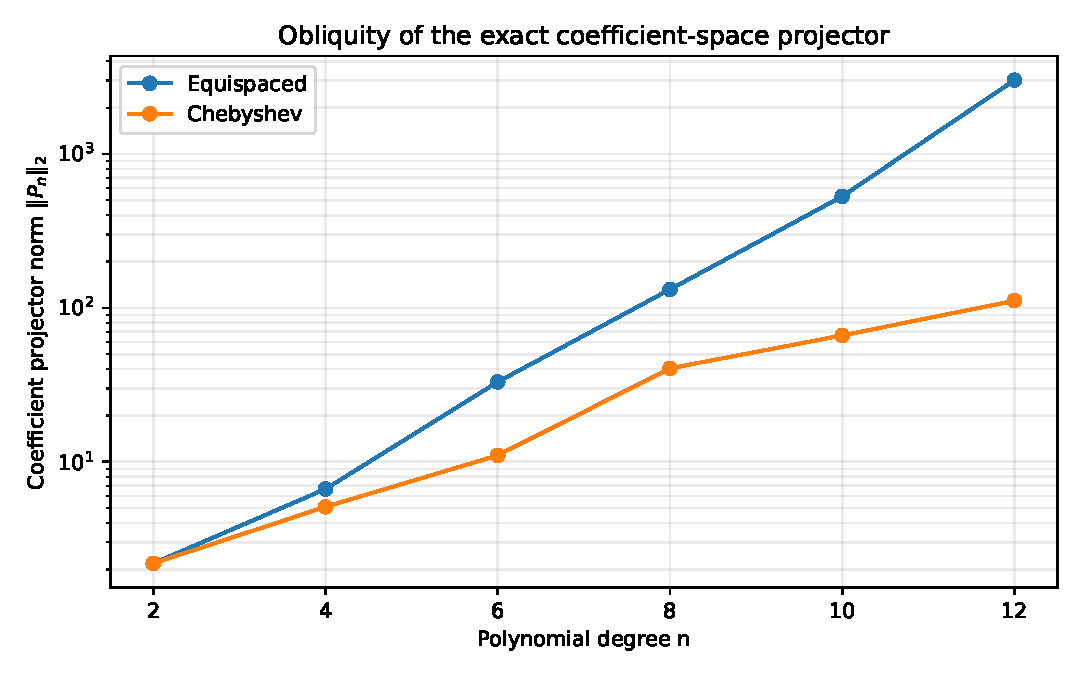
\includegraphics[width=0.92\textwidth]{projector_obliquity.pdf}
\caption{The projector has only the algebraic eigenvalues $0$ and $1$, yet
its largest singular value grows rapidly.  Equispaced nodes make the range
and kernel almost tangent much faster than Chebyshev--Lobatto nodes.}
\label{fig:projector-obliquity}
\end{figure}

The smallest nonzero singular value is numerically close to one in all these
runs, while the largest singular value grows.  This is typical for oblique
projectors: the bad geometry is concentrated in a small number of nearly
parallel range/kernel directions, not in an eigenvalue instability.

\subsection{The loop inherits interpolation error}

The interpolation experiment uses exact dyadic sample values and 140-digit
barycentric arithmetic for the equispaced degrees $32$ and $64$.  Chebyshev
values are evaluated by the stable barycentric formula~\cite{BerrutTrefethen2004}.
The maxima are sampled and refined, not certified continuum extrema.

\begin{table}[htbp]
\centering
\caption{Sampled uniform error for interpolation of $u$ on $[-1,1]$.
By \cref{thm:error-transfer}, these are also exactly the errors of the
corresponding up-shift loop.}
\label{tab:interpolation-errors}
\begin{tabular}{rrr}
\toprule
$n$ & equispaced error & Chebyshev--Lobatto error \\
\midrule
4   & $7.1972\times10^{-2}$ & $8.5439\times10^{-2}$ \\
8   & $2.0217\times10^{-1}$ & $3.5754\times10^{-2}$ \\
16  & $1.9693\times10^{-1}$ & $2.5512\times10^{-3}$ \\
32  & $4.4974\times10^{2}$  & $4.3714\times10^{-4}$ \\
64  & $1.0463\times10^{10}$ & $4.9082\times10^{-6}$ \\
128 & ---                     & $2.6002\times10^{-7}$ \\
\bottomrule
\end{tabular}
\end{table}

The high-precision equispaced peaks occur at approximately
$|x|=0.9859694$ for $n=32$ and $|x|=0.9938615$ for $n=64$, consistent with a
boundary layer of width $\BigO(1/n)$.  The Chebyshev errors are not perfectly
monotone at low degree because $u$ has intricate nonanalytic fine structure,
but the long-range decay is clear.

\begin{figure}[htbp]
\centering
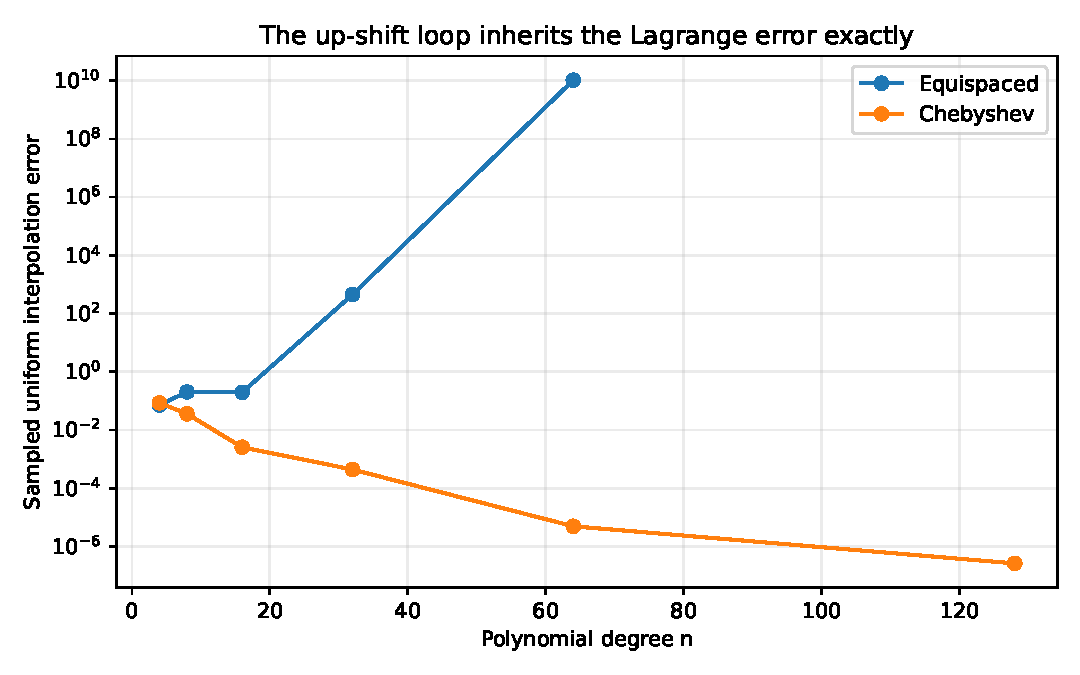
\includegraphics[width=0.92\textwidth]{interpolation_error.pdf}
\caption{Function-space behavior of the closed loop.  The shift synthesis
neither improves nor worsens these curves mathematically: every point is the
error of the original interpolation projector.}
\label{fig:interpolation-error}
\end{figure}

\subsection{Reproducibility files}

Running
\begin{lstlisting}[style=pythonstyle]
python self_representation_experiments.py
\end{lstlisting}
regenerates:
\begin{itemize}
\item \nolinkurl{results/exact_right_inverse_checks.csv};
\item \nolinkurl{results/projector_obliquity.csv};
\item \nolinkurl{results/interpolation_errors.csv};
\item \nolinkurl{results/metadata.json};
\item the two PDF and PNG figures in \nolinkurl{figures/}.
\end{itemize}
The command-line switch \texttt{--quick} omits the degree-$12$ matrices and
the high-precision degree-$64$ endpoint scan.

\section{Further deductions, conjectures, and research directions}
\label{sec:frontiers}

The exact factorization changes the shape of the remaining questions.  The
basic existence problem is solved; the frontier concerns optimal gauges,
conditioning, asymptotics, and structure.

\subsection{Minimal fixed-radius complexity}

\begin{problem}[Arbitrary-shift fixed-radius complexity]
\label{prob:fixed-radius-complexity}
Let $N_n^{(1)}$ be the least number of translates $u(x-\tau_r)$, with
arbitrary real shifts but no dilation, whose span on $[-1,1]$ contains
$\PiN_n$.  Determine the asymptotic growth of $N_n^{(1)}$.
\end{problem}

The general nonpolynomial-atom dimension argument in the synthesis volume
gives $N_n^{(1)}\ge n+2$.  The present uniform-lattice construction and alias
compression give
\begin{equation}
 N_n^{(1)}\le2^{n+1}+n+1.
 \label{eq:N-fixed-bounds}
\end{equation}
For uniform integer-ratio lattices, \cref{prop:lattice-optimal} proves that
the exponential spacing is unavoidable.  What is unknown is whether highly
nonuniform shifts can collapse the count toward the linear lower bound.

\begin{conjecture}[No polynomial-size fixed-radius universal dictionary]
\label{conj:fixed-radius-exponential}
There exists $c>1$ such that $N_n^{(1)}\ge c^n$ for all sufficiently large
$n$.
\end{conjecture}

This conjecture is intentionally labeled speculative.  A possible route is
to combine local non-elementarity with zero-count or Fourier-exponential-type
bounds for finite sums of translates.  A counterexample with $O(n)$
carefully placed centers would be equally interesting and would reveal a
nonuniform analogue of the Rvachev endpoint basis.

\subsection{Asymptotics of projector obliquity}

The equispaced numerical values in \cref{tab:projector-norms} are compatible
with $\log_2\Norm{\Proj_n}_2=n+o(n)$, whereas the Chebyshev sequence is much
smaller over the observed range.

\begin{conjecture}[Equispaced projector exponent]
\label{conj:equi-projector}
For equispaced nodes,
\begin{equation}
 \lim_{n\to\infty}\frac1n\log_2\Norm{\Proj_n}_2=1.
 \label{eq:equi-projector-conj}
\end{equation}
For nested Chebyshev--Lobatto nodes,
$\log\Norm{\Proj_n}_2=o(n)$.
\end{conjecture}

A proof should separate three mechanisms: the classical Lebesgue growth, the
Appell deconvolution symbol $1/\MGF_u$, and exterior evaluation at
$kh\approx\pm2$.  The singular-value problem is only $(n+1)$-dimensional
after reduced QR, so degrees far beyond those in this report are
computationally accessible with matrix-free summation and asymptotic
quadrature.

\subsection{Alias gauges and minimum-variation exact synthesis}

The canonical coefficient vector $\Coeff_np$ is only one representative of
the affine family
\begin{equation}
 \{c:\Synth_nc=p\}=\Coeff_np+\Ker\Synth_n.
 \label{eq:alias-affine-family}
\end{equation}
The explicit confluent Fourier vectors \eqref{eq:alias-vectors} make this a
structured gauge freedom.

\begin{problem}[Optimal exact gauge]
\label{prob:optimal-gauge}
For a chosen norm or weighted norm, find
\begin{equation}
 c_p^\star=\arg\min\{\Norm{c}:\Synth_nc=p\}
 \label{eq:min-gauge}
\end{equation}
and express the minimizing correction to $\Coeff_np$ through the
$q$-integer annihilator $A_n(E)$ or its confluent Fourier basis.  Determine
whether a symmetry-preserving gauge can reduce the exponential coefficient
growth while retaining exact continuum equality.
\end{problem}

This must not be confused with the Moore--Penrose right inverse of the nodal
matrix $B_n$.  The latter gives an orthogonal coefficient projector of norm
one but guarantees only nodal agreement; it need not synthesize the
interpolation polynomial between nodes.  The meaningful optimization is
inside \eqref{eq:alias-affine-family}.

The sign theorem and total-variation bound remain constraints on any
row-unital decoder.  One can formulate a convex program minimizing maximum
negative mass, maximum row variation, or an $\ell^2$ energy while imposing
both exact polynomial reproduction and symmetry.

\subsection{A continuum limit of the signed Markov decoder}

The pair $(\widetilde B_n,D_n)$ resembles a discrete smoothing kernel and its
finite-order inverse.  However, the grid $h=2^{-n}$ becomes exponentially
finer than the node spacing, so the matrices are strongly rectangular.

\begin{question}[Renormalized decoder limit]
Does a rescaling of the row index near the central region or near
$kh=\pm2$ produce a weak limit of the signed measures
\begin{equation}
 \mu_{n,k}=\sum_{j=0}^{n}D_{kj}^{(n)}\delta_{x_j}?
 \label{eq:decoder-measure}
\end{equation}
Can its central limit be described by the inverse differential symbol
$1/\MGF_u$, while its edge limit is controlled by polynomial extrapolation?
\end{question}

For equispaced nodes, the universal lower bound
$V(D_n)\gtrsim n/2$ comes from the total variation of neighboring translated
up densities.  The much larger observed variation suggests a two-scale
decomposition: a local deblurring cost and an exterior cardinal-growth cost.

\subsection{\texorpdfstring{$q$}{q}-binomial minors and Thue--Morse spectral algebra}

The determinant identity \eqref{eq:cauchy-binet} and the zero-mode basis
\eqref{eq:alias-vectors} invite a more explicit $q$-combinatorial treatment.

\begin{problem}[Minor expansion through the annihilator]
Express the minors of $D_n$ after quotienting by $\Ker\Synth_n$ in terms of
coefficients of
\begin{equation}
 A_n(z)=\prod_{r=1}^{n}[2^r]_z
 \label{eq:A-repeat}
\end{equation}
and, where possible, Gaussian binomial coefficients or restricted binary
partition numbers.  Determine whether the Cauchy--Binet sum admits a
sign-reversing involution leaving a small positive residue.
\end{problem}

The exact multiplicity
$2m-n-2=\sum_{j=1}^{m-1}(1+\TwoAdicValuation(j))$ already identifies the projector's
alias zero spectrum with the dyadic zero divisor of $\widehat u$.  A closed
basis for the remaining $2m$ nodal-zero modes might combine Lagrange
vanishing factors with the same cyclotomic blocks.

\subsection{Lambert-\texorpdfstring{$W$}{W} and the Runge boundary layer}

The endpoint values of $F$ and $u$ are governed in the repository by
Lambert-$W$ saddle inversions and log-periodic corrections.  Equispaced
interpolation introduces a second endpoint saddle through binomial
barycentric weights.  The observed peak positions satisfy
$n(1-|x_{\max}|)\approx0.45$ at $n=32$ and $0.39$ at $n=64$.

\begin{conjecture}[Boundary-layer scaling with log-periodic correction]
\label{conj:Runge-layer}
For dyadic equispaced degrees, the dominant symmetric-up Runge peak lies at
\begin{equation}
 1-|x_{\max,n}|=\frac{\alpha(\log_2 n)+o(1)}{n},
 \label{eq:Runge-location-conj}
\end{equation}
where $\alpha$ is bounded and may carry a small periodic modulation inherited
from the dyadic endpoint asymptotics.  The logarithm of the peak amplitude
has an expansion obtained by coupling the binomial saddle with the
Lambert-$W_{-1}$ endpoint saddle of $u$.
\end{conjecture}

A viable derivation would insert the all-orders small-argument expansion of
$F$ into the Newton forward form of the equispaced interpolant, then perform
a two-parameter saddle analysis in the node index and boundary-layer
coordinate.  This directly connects the inverse-Fabius/Lambert-$W$ corpus to
the present transform.

\subsection{Node sets co-designed with the up kernel}

Classical node selection minimizes polynomial interpolation growth.  The
factorization suggests a stronger objective involving both the Lagrange
space and the up dictionary, for example
\begin{equation}
 \min_{X_n}\Norm{D_n(X_n)\widetilde B_n(X_n)}_2,
 \quad
 \min_{X_n}V(D_n(X_n)),
 \quad\text{or}\quad
 \max_{X_n}\theta_n.
 \label{eq:node-design}
\end{equation}
The minimizers need not be exactly Chebyshev points: the positive kernel
$u(x_i-kh)$ introduces a scale-dependent geometry absent from ordinary
Lebesgue optimization.  Up-adapted Fekete or Leja points are a promising
computational frontier.

\subsection{Formalization}

Most identities after \cref{thm:fixed-radius} are finite-dimensional and
well suited to Lean:
\begin{enumerate}
\item define the terminating operator $\App$ on \texttt{Polynomial};
\item import or formalize the fixed-radius affine conjugation of the existing
synthesis theorem;
\item construct the Lagrange basis and prove $B_nC_n=I$;
\item derive idempotence, rank, direct sums, and the nested projector algebra;
\item formalize the Markov-overlap sign theorem independently of analysis;
\item connect the alias kernel to the existing Thue--Morse and valuation
lemmas.
\end{enumerate}
The exact degree-$2$, $4$, and $8$ rational checks can serve as executable
regression certificates.

\section{Conclusion}
\label{sec:conclusion}

The requested loop closes cleanly once the synthesis theorem is viewed
through affine conjugation.  Degree-$n$ polynomial reproduction at scale
$2^n$ is the same statement as fixed-radius reproduction by spacing-$2^{-n}$
translates.  Applying the resulting inverse-moment Appell sampler to every
Lagrange cardinal yields an explicit finite matrix $D_n$; applying it after
interpolation yields the canonical self-amplitudes
\[
 c_{n,k}=2^{-n}[\MGF_u(D)^{-1}\Lag_nu](k2^{-n}).
\]
The apparent self-representation operator is exactly the ordinary Lagrange
projector in different coordinates.

That exactness is both the strength and the warning.  It provides a right
inverse, a Markov/signed-Markov factorization, a complete two-point spectrum,
a $2$-adic alias multiplicity formula, an exact local direct sum, and a
nested dyadic spectral flag.  It also proves that the transformation cannot
suppress Runge's phenomenon: stable nodes remain stable, unstable nodes
remain unstable, and every fixed-level truncation is already exact.  The new
mathematics lies in the coefficient geometry---alias gauges, oblique angles,
negative mass, extrapolation growth, and the distinction between nodal and
continuum exactness.

The most promising next step is to optimize within the explicit alias
nullspace.  A minimum-variation, symmetry-preserving exact gauge could retain
the conceptual elegance of literal up shifts while substantially reducing
the enormous canonical coefficients.  In parallel, the equispaced boundary
layer offers a concrete meeting point for the repository's Lagrange,
Thue--Morse, Fourier-decay, and Lambert-$W$ asymptotic machinery.

\appendix

\section{Formula sheet}
\label{app:formula-sheet}

For quick reference, the complete canonical transform is:
\begin{align}
 m&=2^n,\qquad h=2^{-n},
 \label{eq:sheet-scale}\\
 K_n&=\{-2m+1,\ldots,2m-1\},
 \label{eq:sheet-grid}\\
 \frac1{\MGF_u(z)}
 &=\exp\!\left[-\sum_{r\ge1}
   \frac{B_{2r}}{2r(1-4^{-r})}\frac{z^{2r}}{(2r)!}\right]
 =\sum_{r\ge0}\gamma_r\frac{z^r}{r!},
 \label{eq:sheet-gamma}\\
 \App p&=\sum_{r=0}^{\Floor{\deg p/2}}
 \frac{\gamma_{2r}}{(2r)!}p^{(2r)},
 \label{eq:sheet-App}\\
 D_{kj}^{(n)}&=(\App\ell_j)(kh)
 =\frac1{\omega_n'(x_j)}
   \sum_{r=0}^{\Floor{n/2}}\gamma_{2r}
   e_{n-2r}(\{kh-x_s:s\ne j\}),
 \label{eq:sheet-D}\\
 \ell_j(x)&=h\sum_{k\in K_n}D_{kj}^{(n)}u(x-kh),
 \label{eq:sheet-cardinal}\\
 c_k(y)&=h\sum_{j=0}^{n}D_{kj}^{(n)}y_j,
 \label{eq:sheet-c}\\
 \Rec_ny&=\sum_{k\in K_n}c_k(y)u(\cdot-kh),
 \label{eq:sheet-loop}\\
 \widetilde B_{ik}&=hu(x_i-kh),
 &\widetilde B_nD_n&=I_{n+1},
 &\Proj_n&=D_n\widetilde B_n,
 \label{eq:sheet-matrices}\\
 \chi_{\Proj_n}(\lambda)
 &=\lambda^{4\cdot2^n-n-2}(\lambda-1)^{n+1}.
 \label{eq:sheet-spectrum}
\end{align}

\section{Dimension and multiplicity ledger}
\label{app:ledger}

\begin{longtable}{@{}p{0.42\textwidth}p{0.18\textwidth}p{0.30\textwidth}@{}}
\caption{Exact dimensions for degree $n$, $m=2^n$.}\label{tab:dimension-ledger}\\
\toprule
Object & Dimension & Interpretation \\
\midrule
\endfirsthead
\toprule
Object & Dimension & Interpretation \\
\midrule
\endhead
Dense fixed-radius coefficient space & $4m-1$ & all active $h\IntegerNumbers$ shifts on $[-1,1]$ \\
Local up-shift function space $\mathcal V_n$ & $2m+n+1$ & imported multi-cell dimension \\
Polynomial subspace $\PiN_n$ & $n+1$ & one-eigenspace of the loop projector \\
Nodal-zero local space $\mathcal Z_n$ & $2m$ & nonzero up-splines invisible at nodes \\
Dense alias kernel $\Ker\Synth_n$ & $2m-n-2$ & confluent dyadic Fourier modes \\
Dense sample kernel $\Ker B_n$ & $4m-n-2$ & full zero-eigenspace of $\Proj_n$ \\
Compressed coefficient basis & $2m+n+1$ & alias-free right-end shift basis \\
Compressed projector zero eigenspace & $2m$ & only the nodal-zero sector remains \\
\bottomrule
\end{longtable}

\section{Notes on numerical verification}
\label{app:numerical-notes}

The exact arithmetic path is deliberately independent of the Fourier path.
For $n=1,2,4,8$:
\begin{enumerate}
\item $\gamma_r$ are generated symbolically from the Bernoulli cumulant
series;
\item Lagrange cardinals are multiplied over \texttt{Fraction};
\item $D_n$ is evaluated by exact derivatives and Horner evaluation;
\item Fabius values at dyadic rationals are generated by the terminating
highest-bit recursion;
\item $u(t)=F(1-|t|)$ evaluates every entry of $\widetilde B_n$ exactly;
\item the matrix product is performed over $\RationalNumbers$.
\end{enumerate}
The Fourier cosine evaluator is used only for non-dyadic floating-point
nodes, plots, and larger projector diagnostics.  This separation makes it
unlikely that a shared implementation error could manufacture
$\widetilde B_nD_n=I$.

\section{Selected corpus crosswalk}
\label{app:crosswalk}

\begin{longtable}{@{}p{0.29\textwidth}p{0.63\textwidth}@{}}
\caption{Repository material used to set notation and avoid duplication.}
\label{tab:crosswalk}\\
\toprule
Corpus branch & Role in this report \\
\midrule
\endfirsthead
\toprule
Corpus branch & Role in this report \\
\midrule
\endhead
Primary exposition & Definitions of $F$ and $u$, functional equations,
probability model, sinc product, moments, dyadic arithmetic. \\
Up polynomial synthesis & Imported Strang--Fix scale classification, global
Appell deconvolution, local dimension, alias annihilator, endpoint and
multi-cell bases, fast coefficient algorithm. \\
Dyadic-comb frontiers & Imported Lagrange/Hermite interpolation setup,
symmetry reductions, Lebesgue/Runge analysis, exact dyadic numerical data. \\
Representation frontiers & Fourier, Faber--Schauder, Bernstein, Bessel, and
multiresolution formulas; independent cosine evaluator used by the
experiments. \\
Thue--Morse atlas/frontiers & Prouhet cancellation, dyadic products, finite
block calculus, valuation multiplicities. \\
Exponent and $q$-series frontiers & $q$-Pochhammer, Gaussian-binomial,
Bernoulli--Bell expansions, finite sinc approximants and transport geometry. \\
Inverse and sampling frontiers & Inverse-Fabius asymptotics, sampling
operators, endpoint structure, Lambert-$W$ inversion. \\
Spectra and arithmetic frontiers & Spectral multiplicities, exact rational
structures, and matrix viewpoints compared against the projector results. \\
Fourier-decay corpus & Log-Gaussian envelope and periodic modulation relevant
to sharp Chebyshev and boundary-layer asymptotics. \\
Lean walkthrough & Existing formal definitions and theorem dependency graph
for future formalization. \\
Paper transcriptions & Historical and published sources on Fabius/up
arithmetic, lacunary products, and related functional equations. \\
Archive & Frozen derivations and predecessor reports used for provenance and
to avoid re-claiming absorbed formulas. \\
\bottomrule
\end{longtable}

\begin{thebibliography}{99}

\bibitem{Fabius1966}
J.~Fabius,
\newblock A probabilistic example of a nowhere analytic $C^\infty$-function,
\newblock \emph{Zeitschrift f\"ur Wahrscheinlichkeitstheorie und Verwandte
Gebiete} \textbf{5} (1966), 173--174.

\bibitem{RvachevRvachev1971}
V.~L.~Rvachev and V.~A.~Rvachev,
\newblock A certain finite function,
\newblock \emph{Dopovidi Akademii Nauk Ukrains'koi RSR, Series A} (1971),
705--707, 764.

\bibitem{RvachevRvachev1972}
V.~L.~Rvachev and V.~A.~Rvachev,
\newblock On the representation of polynomials by functions with compact
support,
\newblock \emph{Mathematical Physics}, No.~11, Naukova Dumka, Kiev, 1972,
126--129.

\bibitem{Rvachev1977}
V.~A.~Rvachev,
\newblock On approximation by means of the function $\RvachevUp(x)$,
\newblock \emph{Doklady Akademii Nauk SSSR} \textbf{233} (1977), no.~2,
295--296.

\bibitem{Rvachev1990}
V.~A.~Rvachev,
\newblock Compactly supported solutions of functional-differential equations
and their applications,
\newblock \emph{Russian Mathematical Surveys} \textbf{45} (1990), no.~1,
87--120.

\bibitem{Arias1982}
J.~Arias de Reyna,
\newblock Definici\'on y estudio de una funci\'on indefinidamente
diferenciable de soporte compacto,
\newblock \emph{Revista de la Real Academia de Ciencias Exactas, F\'isicas y
Naturales de Madrid} \textbf{76} (1982), 21--38; English translation
arXiv:1702.05442.

\bibitem{Arias2018}
J.~Arias de Reyna,
\newblock Arithmetic of the Fabius function,
\newblock \emph{INTEGERS} \textbf{18} (2018), Article A51.

\bibitem{StrangFix1973}
G.~Strang and G.~Fix,
\newblock A Fourier analysis of the finite element variational method,
\newblock in \emph{Constructive Aspects of Functional Analysis}, C.I.M.E.,
1973, 793--840.

\bibitem{deBoorRon1992}
C.~de~Boor and A.~Ron,
\newblock Fourier analysis of the approximation power of principal
shift-invariant spaces,
\newblock \emph{Constructive Approximation} \textbf{8} (1992), 427--462.

\bibitem{deBoorDeVoreRon1994}
C.~de~Boor, R.~A.~DeVore, and A.~Ron,
\newblock Approximation from shift-invariant subspaces of
$L_2(\RealNumbers^d)$,
\newblock \emph{Transactions of the American Mathematical Society}
\textbf{341} (1994), 787--806.

\bibitem{Jia1998}
R.-Q.~Jia,
\newblock Shift-invariant spaces and linear operator equations,
\newblock \emph{Israel Journal of Mathematics} \textbf{103} (1998),
259--288.

\bibitem{Roman1984}
S.~Roman,
\newblock \emph{The Umbral Calculus},
\newblock Academic Press, 1984.

\bibitem{Comtet1974}
L.~Comtet,
\newblock \emph{Advanced Combinatorics},
\newblock Reidel, 1974.

\bibitem{AlloucheShallit2003}
J.-P.~Allouche and J.~Shallit,
\newblock \emph{Automatic Sequences: Theory, Applications,
Generalizations},
\newblock Cambridge University Press, 2003.

\bibitem{BerrutTrefethen2004}
J.-P.~Berrut and L.~N.~Trefethen,
\newblock Barycentric Lagrange interpolation,
\newblock \emph{SIAM Review} \textbf{46} (2004), no.~3, 501--517,
DOI 10.1137/S0036144502417715.

\bibitem{Higham2004}
N.~J.~Higham,
\newblock The numerical stability of barycentric Lagrange interpolation,
\newblock \emph{IMA Journal of Numerical Analysis} \textbf{24} (2004),
547--556.

\bibitem{PlatteTrefethenKuijlaars2011}
R.~B.~Platte, L.~N.~Trefethen, and A.~B.~J.~Kuijlaars,
\newblock Impossibility of fast stable approximation of analytic functions
from equispaced samples,
\newblock \emph{SIAM Review} \textbf{53} (2011), no.~2, 308--318,
DOI 10.1137/090774707.

\bibitem{Trefethen2013}
L.~N.~Trefethen,
\newblock \emph{Approximation Theory and Approximation Practice},
\newblock SIAM, 2013.

\bibitem{ProveItPrimary}
V.~Reshetnikov,
\newblock \emph{The Fabius Function and Rvachev's Up-Function},
\newblock primary exposition in the \texttt{ProveIt} repository,
\repo, snapshot commit
\nolinkurl{4544e9af6b94820402c69967be1dff3f85e43c1e}, 2026.

\bibitem{ProveItSynthesis}
V.~Reshetnikov,
\newblock \emph{Exact Polynomial Synthesis by Finite Rvachev Up-Function
Dictionaries},
\newblock \nolinkurl{semi-formalized-research-frontiers/drafts/representations/Up_Polynomial_Synthesis/},
\texttt{ProveIt} snapshot commit
\nolinkurl{4544e9af6b94820402c69967be1dff3f85e43c1e}, 2026.

\bibitem{ProveItDyadicComb}
V.~Reshetnikov,
\newblock \emph{Dyadic-Comb Frontiers for the Fabius--Rvachev System},
\newblock \nolinkurl{semi-formalized-research-frontiers/drafts/inverse-and-sampling/comb-interpolation/Dyadic_Comb_Frontiers/},
\texttt{ProveIt} snapshot commit
\nolinkurl{4544e9af6b94820402c69967be1dff3f85e43c1e}, 2026.

\bibitem{ProveItRepresentation}
V.~Reshetnikov,
\newblock \emph{Representation Frontiers for the Fabius--Rvachev System},
\newblock consolidated frontier volume in \texttt{ProveIt}, snapshot commit
\nolinkurl{4544e9af6b94820402c69967be1dff3f85e43c1e}, 2026.

\bibitem{ProveItInverse}
V.~Reshetnikov,
\newblock \emph{Inverse and Sampling Frontiers for the Fabius--Rvachev
System},
\newblock consolidated frontier volume in \texttt{ProveIt}, snapshot commit
\nolinkurl{4544e9af6b94820402c69967be1dff3f85e43c1e}, 2026.

\end{thebibliography}

\end{document}
% Canonical mathematical notation for active FabiusFunction LaTeX documents.
%
% This file is intentionally a plain TeX input rather than a LaTeX package.
% Every standalone document loads it by an explicit path relative to that
% document's directory; included fragments inherit the definitions from their
% root document.  Keep this file independent of document layout and metadata.
%
% Contract:
%   * one command has one mathematical meaning throughout the active corpus;
%   * names encode semantic roles rather than a document-local choice of letter;
%   * visually similar but differently normalized objects have different print;
%   * every command below is defined normatively in the notation catalogue.
%
% The active corpus excludes docs/archive/.  Historical sources may retain
% their original notation only inside an explicitly labelled quotation.

\makeatletter
\@ifundefined{mathbb}{%
  \PackageError{fabius-notation}{The amssymb package must be loaded first}%
    {Load amsmath and amssymb before inputting fabius-notation.tex.}%
}{}
\@ifundefined{operatorname}{%
  \PackageError{fabius-notation}{The amsmath package must be loaded first}%
    {Load amsmath before inputting fabius-notation.tex.}%
}{}
\makeatother

% Version stamp used by the catalogue and by static audits.
\newcommand{\FabiusNotationVersion}{2026-08-31}

% Number systems.  NaturalNumbers is explicitly the nonnegative convention.
\newcommand{\NaturalNumbers}{\mathbb{N}_{0}}
\newcommand{\PositiveIntegers}{\mathbb{N}_{>0}}
\newcommand{\IntegerNumbers}{\mathbb{Z}}
\newcommand{\RationalNumbers}{\mathbb{Q}}
\newcommand{\RealNumbers}{\mathbb{R}}
\newcommand{\ComplexNumbers}{\mathbb{C}}
\newcommand{\ExtendedRealNumbers}{\overline{\mathbb{R}}}

% The three principal Fabius--Rvachev functions.  Subscripts are deliberate:
% a bare F and a calligraphic F have several unrelated uses in the corpus.
\newcommand{\FabiusBounded}{F_{\mathrm{bd}}}
\newcommand{\FabiusGlobal}{F_{\mathrm{gl}}}
\newcommand{\FabiusQuantile}{Q_{F}}
\newcommand{\FabiusClampedQuantile}{Q_{F,\mathrm{cl}}}
\newcommand{\RvachevUp}{\operatorname{up}}

% Constants, elementary operators, and delimiters.
\newcommand{\EulerE}{\mathrm{e}}
\newcommand{\ImaginaryUnit}{\mathrm{i}}
\newcommand{\Differential}{\mathop{}\!\mathrm{d}}
\newcommand{\AbsoluteValue}[1]{\left\lvert #1\right\rvert}
\newcommand{\Norm}[1]{\left\lVert #1\right\rVert}
\newcommand{\Floor}[1]{\left\lfloor #1\right\rfloor}
\newcommand{\Ceiling}[1]{\left\lceil #1\right\rceil}
\newcommand{\FractionalPart}[1]{\left\{#1\right\}}
\newcommand{\PositivePart}[1]{\left(#1\right)_{+}}
\newcommand{\IndicatorOf}[1]{\mathbf{1}_{#1}}
\newcommand{\SetOf}[1]{\left\{#1\right\}}
\newcommand{\InnerProduct}[1]{\left\langle #1\right\rangle}
\newcommand{\CardinalityOf}[1]{\left\lvert #1\right\rvert}
\newcommand{\DefinitionEquals}{\mathrel{\coloneqq}}
\newcommand{\Sign}{\operatorname{sgn}}
\newcommand{\IdentityOperator}{\operatorname{id}}
\newcommand{\SpanOperator}{\operatorname{span}}
\newcommand{\TraceOperator}{\operatorname{tr}}
\newcommand{\RankOperator}{\operatorname{rank}}
\newcommand{\DiagonalOperator}{\operatorname{diag}}
\newcommand{\ResidueOperator}{\operatorname*{Res}}
\newcommand{\LeastCommonMultiple}{\operatorname{lcm}}
\newcommand{\OrderOperator}{\operatorname{ord}}
\newcommand{\PrincipalLogarithm}{\operatorname{Log}}
\newcommand{\FallingFactorial}[2]{\left(#1\right)^{\underline{#2}}}
\newcommand{\RisingFactorial}[2]{\left(#1\right)^{\overline{#2}}}

% Support, topology, convolution, and metric notation.
\newcommand{\SupportOperator}{\operatorname{supp}}
\newcommand{\SupportOf}[1]{\SupportOperator\!\left(#1\right)}
\newcommand{\TopologicalSupportOf}[1]{\operatorname{tsupp}\!\left(#1\right)}
\newcommand{\Convolution}{\mathbin{*}}
\newcommand{\MetricDistance}{\operatorname{dist}}
\newcommand{\TotalVariationDistance}{d_{\mathrm{TV}}}

% Probability.  Equality and convergence in law are not metric distance.
\newcommand{\Probability}{\mathbb{P}}
\newcommand{\Expectation}{\mathbb{E}}
\newcommand{\Variance}{\operatorname{Var}}
\newcommand{\Covariance}{\operatorname{Cov}}
\newcommand{\LawOperator}{\operatorname{Law}}
\newcommand{\LawOf}[1]{\LawOperator\!\left(#1\right)}
\newcommand{\EqualInLaw}{\mathrel{\overset{\mathrm{law}}{=}}}
\newcommand{\ConvergesInLaw}{\mathrel{\xrightarrow{\mathrm{law}}}}

% Fourier and integral transforms.  The printed labels expose normalization.
% FourierTwoPi uses exp(-2*pi*i*x*xi); FourierAngular uses exp(-i*x*omega).
\newcommand{\FourierTwoPi}[1]{\widehat{#1}_{\,2\pi}}
\newcommand{\FourierAngular}[1]{\widehat{#1}_{\,\mathrm{ang}}}
\newcommand{\LaplaceTransformSymbol}{\mathcal{L}}
\newcommand{\MellinTransformSymbol}{\mathcal{M}}
\newcommand{\LaplaceTransformOf}[1]{\LaplaceTransformSymbol\!\left[#1\right]}
\newcommand{\MellinTransformOf}[1]{\MellinTransformSymbol\!\left[#1\right]}
\newcommand{\MomentGeneratingFunction}[1]{M_{#1}}
\newcommand{\CharacteristicFunction}[1]{\varphi_{#1}}

% The two standard sinc functions must never share one symbol.
\newcommand{\SincRad}{\operatorname{sinc}_{\mathrm{rad}}}
\newcommand{\SincPi}{\operatorname{sinc}_{\pi}}

% Binary arithmetic and Thue--Morse notation.
\newcommand{\BinaryDigitSum}{\operatorname{wt}_{2}}
\newcommand{\ThueMorseSignSymbol}{\varepsilon}
\newcommand{\ThueMorseSign}[1]{\varepsilon_{#1}}
\newcommand{\PadicValuation}[1]{\nu_{#1}}
\newcommand{\TwoAdicValuation}{\nu_{2}}

% q-series notation.  Every base is an explicit argument.
\newcommand{\QPochhammer}[3]{\left(#1;#2\right)_{#3}}
\newcommand{\GaussianBinomial}[3]{%
  \genfrac{[}{]}{0pt}{}{#1}{#2}_{#3}%
}
\newcommand{\QInteger}[2]{\left[#1\right]_{#2}}

% Named special functions.
\newcommand{\Polylogarithm}{\operatorname{Li}}
\newcommand{\LambertW}{W}
\newcommand{\GammaFunction}{\Gamma}
\newcommand{\RiemannZeta}{\zeta}

% Asymptotics.  BigO and LittleO are operator tokens for existing formula
% grammar; prefer the At forms so that the limiting regime is printed.
\newcommand{\BigO}{\mathcal{O}}
\newcommand{\LittleO}{o}
\newcommand{\BigOAt}[2]{\mathcal{O}_{#2}\!\left(#1\right)}
\newcommand{\LittleOAt}[2]{o_{#2}\!\left(#1\right)}

